\chapter{Waypoint Flow Regulator}
\label{chap5}
The complementary algorithm to the Airport Flow Regulator (AFR), is the Waypoint Flow Regulator (WFR), both of which work together to achieve the goal of regulating aircraft flow in the context of Air Traffic Flow Management (ATFM). We recall from Section \ref{sec:WFR}, the goal of the WFR is to issue speed regulation and hold commands to aircraft such that the minimum required separation between any pair of aircraft at all nodes are observed. We also penalize deviations from the preferred time to exit the current FIR, denoted backTTO, and holding times according to the node type. 

This work begins at the construction of the network of air navigation routes for the ASEAN Plus region, based on flight schedules (departure and arrival times) obtained from OAG \parencite{OAG2024a}. We build the network of nodes and routes by (i) processing information from the Aeronautical Information Publication (AIP) documents published by each country's civil aviation authority to identify the nodes (or waypoints) (see Figure \ref{fig:nodes}), and arcs connecting waypoints along routes (see Figure \ref{fig:arcs}) (ii) applying Dijkstra's algorithm to determine the shortest path between any airport pair, thereby defining the flight path routing for each flight.

\begin{figure}
    \centering
    \includegraphics[width=0.8\textwidth]{Figures/FIR nodes.png}
    \caption{Flight Network Nodes Within the ASEAN Plus Region, with FIR Boundaries}
    \label{fig:nodes}
\end{figure}

\begin{figure}
    \centering
    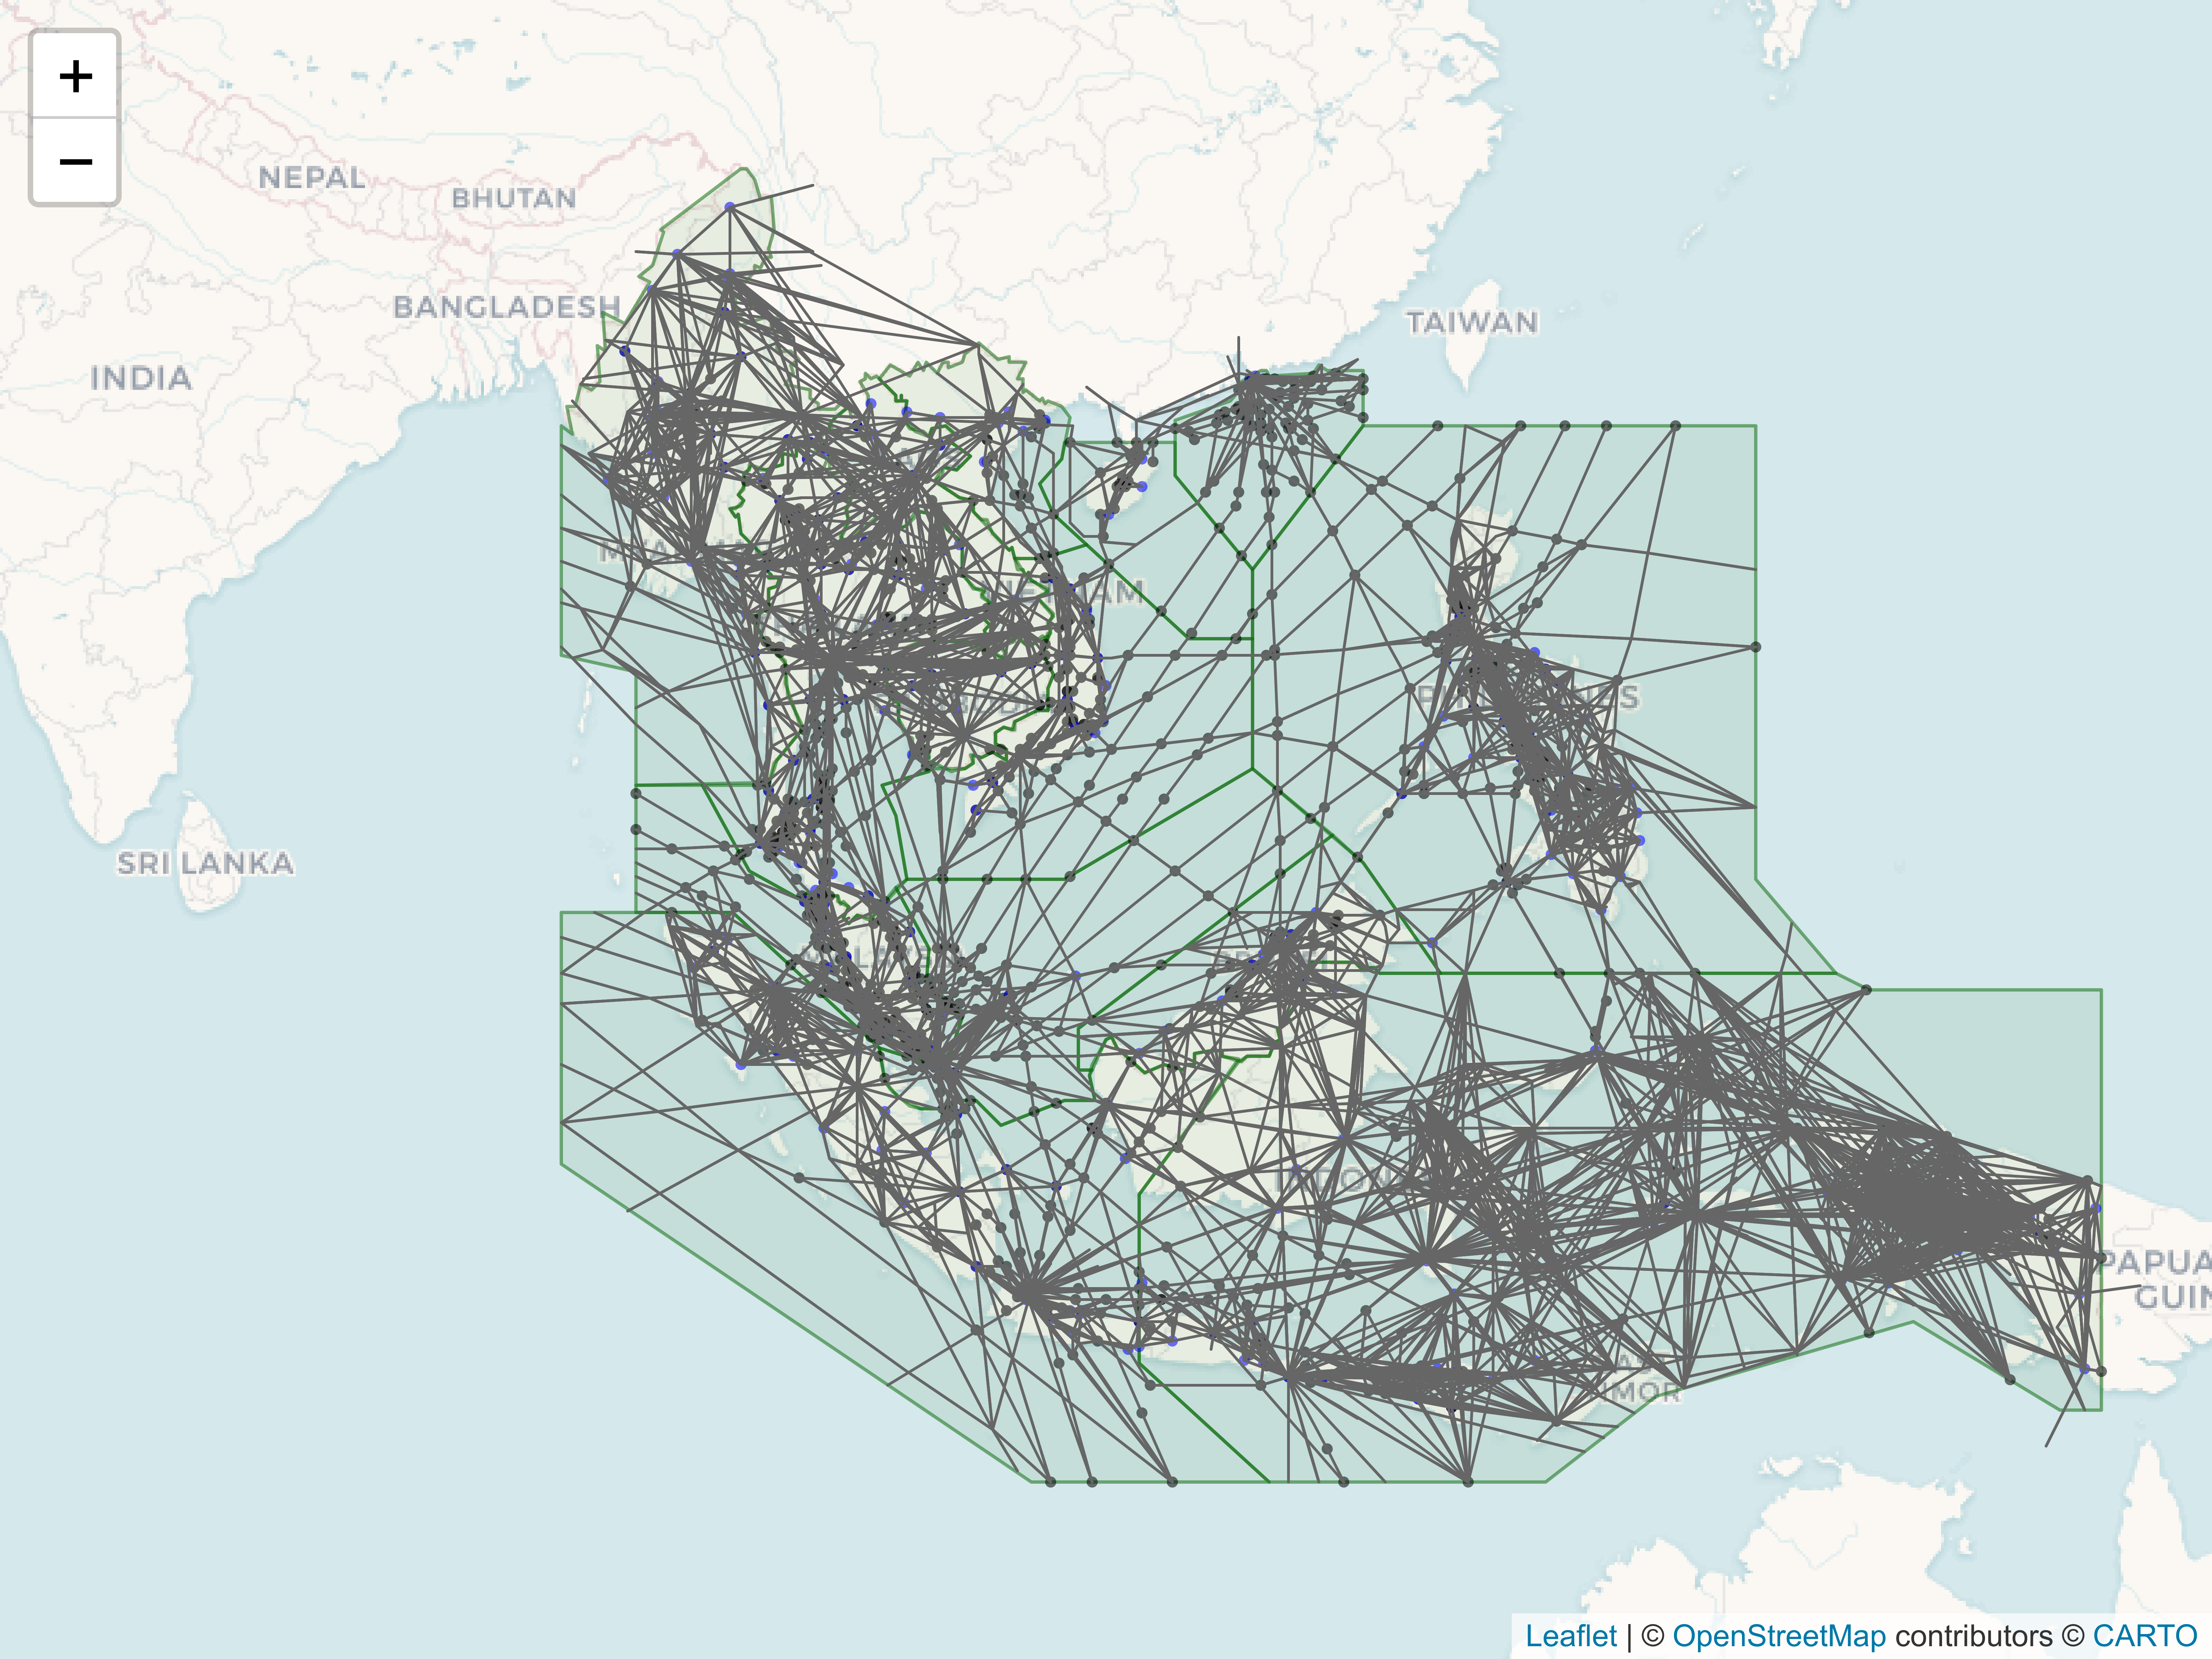
\includegraphics[width=0.8\textwidth]{Figures/FIR arcs.png}
    \caption{Flight Network Arcs Within the ASEAN Plus Region, with FIR Boundaries}
    \label{fig:arcs}
\end{figure}

We first formulate the optimization problem mathematically and provide a brief overview of the concepts central to mathematical optimization. Subsequently, we propose two algorithms to solve this problem, namely, Gradient Descent Ascent (GDA) and Simulated Annealing (SA). The formulations, results and additional considerations are included for each algorithm. Lastly, a summary of notation used in this chapter is provided in Section \ref{sec:WFRnotation}.

%--------------------------------------------------------
\section{Mathematical Formulation}
\label{sec:MF}
For each input dataset, we are given the initial flight trajectory for all flights in a single Flight Information Region (FIR). A flight trajectory consists of the path a flight will take, from entry to exit of this FIR, and the entry time of a flight into this FIR. We base our dataset on flight schedules (arrival and departure times) downloaded from OAG \parencite{OAG2024a}, and on flight plans derived using Dijkstra's shortest path algorithm applied to a representative network we created of air navigation routes for the ASEAN Plus region with connections to all origin-destination pairs in the flight schedule. Each flight plan specifies the sequence of nodes in our network traversed from its departure airport to its arrival airport. A node in the regional network may represent either an airport or a waypoint. For notational convenience, since the channels have been earlier determined by the AFR, a node in this chapter may refer to a waypoint, or a channel, one of arrival, departure, or mixed, at an airport. Each node in the regional network is designated by the FIR to which it belongs. Let $\mathcal{N}$ denote the set of nodes for the FIR of interest. For the FIR of interest, and each flight in the schedule, we restrict attention to the portion of the flight plan visiting nodes within that FIR. Let $\mathcal{F}$  denote the set of flight plans which intersect with $\mathcal{N}$. Let $P_f$ denote the sequence of nodes for flight $f\in\mathcal{F}$. We assume that the sequence is contiguous in terms of flight legs, that is, a flight does not leave an FIR and then re-enter the same FIR on a later leg of its journey. Let $j=1,2,\cdots,|P_f|$ index the nodes of the FIR-restricted flight plan in sequence and let $n_j\in\mathcal{N}$, or simply $n\in\ P_f$ when no confusion should exist, denote a particular node in the sequence.

We assume that each flight $f$ has an earliest time, $t_f^0$, at which it is estimated or known to have entered the airspace of the FIR. This could be the scheduled or actual departure time from an airport within the FIR, or it could be the estimated or known time the flight traversed the last node of a flight plan in an adjacent FIR, prior to entering the FIR of interest. Accordingly, we append a node $j=0$ to the beginning of each flight plan $P_f$ and associate with it the fixed time, $t_f^0$. No decision variables are associated with this node, so $n_0$ affects only the right-hand side of a constraint.

Similarly, we assume that each flight has a target time to land or otherwise exit the FIR. We associate this time with the last node in the flight plan and designate it as $\widetilde{t}_{|Pf|}$. In our simulation model, such times are initialized using flight schedules and updated dynamically by the airport flow regulator algorithm (for arrival times within the FIR) or, depending on the information sharing regime, passed in from the neighboring FIR if the flight transits out of the FIR of interest.

Each node $j=1,2,\cdots,|P_f|$, marks the \textit{end} of a flight leg. The first leg, $j=1$, can be thought of as the trip from the departure gate to the runway of the origin airport. We assume that the leg from $n_{j-1}$ to $n_j$ has a preferred duration ${\widetilde{d}}_{fj}$ particular to the flight $f$. The preferred duration of the first leg is zero (${\widetilde{d}}_{f1}=0$). In our simulation, we compute an ideal time profile for each trajectory as a whole from origin to destination with reference to the rate of ascent, cruising altitude, cruising speed, and rate of descent specific to the equipment type.  We compute an upper time profile (resp. lower time profile) by scaling the cruising speed down by 10\% (resp. up by 5\%).  For any leg, we use these three profiles to derive the preferred duration ${\widetilde{d}}_{fj}$, as well as the maximum ${\overline{d}}_{fj}$, and minimum ${\underline{d}}_{fj}$ leg durations. Appendix \ref{AppendixB} documents the calculations.

The trajectory of each flight $f\in\mathcal{F}$ is determined by the flight plan $P_f$, and for each node $j=1,2,\cdots,|P_f|$, the target time over (TTO) at the $j^{th}$ node in path $P_f$, denoted by $t_{fj}$.

For each node $j=1,2,\cdots,|P_f|$, we introduce two decision variables: a speed regulation factor, $\beta_{fj}$, and an extraordinary hold delay, $h_{fj}$. The TTO values are determined with the following forward recursion:
\begin{equation}
\label{eqn:fwrec1}
t_{f0}=t_f^0;
\end{equation}
\begin{equation}
\label{eqn:fwrec2}
t_{fj}=t_{fj-1}+h_{fj}+\beta_{fj}{\underline{d}}_{fj}+(1-\beta_{fj}){\overline{d}}_{fj};
\end{equation}
where $h_{fj}\geq0$ and $0\le\beta_{fj}\le1$ for all $j=1,2,\cdots,|P_f|$. Observe that increasing the speed regulation factor, $\beta_{fj}$, is associated with \textit{reducing} the duration of the $j^{th}$ leg. 

Also, observe that the extraordinary hold delay, $h_{fj}$, is applied to the trajectory after the flight has traversed node $j-1$. Thus, if we consider the first node in the FIR network, $j=1$, then the first node in the flight path, $j=0$, is a dummy node representing either a node in an adjacent FIR or an airport departure node. Consequently, $h_{f1}$ can be interpreted as a request to the neighboring FIR to hold a flight from entering the FIR of interest or a request to the airport scheduler to impose an additional ground delay on the flight.

We impose no upper limits on the extraordinary hold delay variables, $h_{fj}$. Instead, we introduce an extraordinary hold cost parameter $c_n$ associated with nodes $n\in\mathcal{N}$ to be applied to these delays. We anticipate the traffic manager would designate five classes of nodes with progressively increasing cost parameters: airport nodes (for which delays represent ground delays which cost less than airborne delays), neighboring FIR nodes (for which delays represent external airborne holding or requests for collaborative ground delays), nodes at entrances to designated holding areas within the FIR of interest, final approach nodes (for which delays represent vectoring), and all other waypoints (for which delays are strongly discouraged). In the experiments reported below, for example, we set the default values for holding costs for departure airports and final approach nodes at 1 and 10, respectively. Holding costs at all other nodes were set at 100.

The decision problem becomes a flow regulation problem when we impose flow constraints on the number of aircraft traversing specific nodes in the network. The flow capacity, and by extension, the minimum required separation time at each node, is determined in the same manner as in Section \ref{sec:envelope}. We consider simple flow constraints, such as an upper bound on the number of traversals by aircraft of any type through a given node during the current planning horizon. We enforce this by imposing a minimum separation time between any pair of flights whose flight path takes them through the constrained node. We let $\Delta_n$ denote the minimum separation time for flights traversing the node $n$.

To express the flow constraint generically, let $n$ denote a node with a flow constraint and let $f$ and $f'$ denote any pair of flights whose flight paths both include the node $n$. Let $j$ index node $n$ in $P_f$ and let $j'$ index node $n$ in $P_{f'}$. Let $\mathcal{C}$ denote the set of all such tuples $(f,f^\prime,j,j')$ of potential conflicts. Denote the corresponding TTOs at this node for these flights by $t_{fj}$ and $t_{f^\prime j^\prime}$, respectively. We require $\left|t_{fj}-t_{f^\prime j^\prime}\right|\geq\Delta_n$. We enforce this generically by defining a penalty function $\delta\left(\left|t_{fj}-t_{f^\prime j^\prime}\right|\right)$ for any strictly decreasing function $\delta(\cdot)$ and imposing the constraint:
\begin{equation}
    \delta\left(\left|t_{fj}-t_{f^\prime j^\prime}\right|\right)\le\delta\left(\Delta_n\right),
\end{equation}
where $n=n_j=n_{j^\prime}$.

An additional complication arises from the fact that these trajectories are updated in a rolling horizon fashion. At any point in time, some of the flights are en route. Consequently, not all TTOs are free to be modified. Our convention is that the TTO for the ending node of a leg becomes \textit{frozen} as soon as the simulation clock exceeds the TTO of the beginning node of that leg. That is, once an aircraft has transited a node, the TTO of the next node in its flight plan is frozen in time. The following proposition follows, which is a necessary condition for the forward TTO recursion.

\begin{proposition}
\label{prop:frozen}
    For any given trajectory, there does not exist a free leg before a frozen leg.
\end{proposition}
\begin{proof}
    From the definition of a frozen leg, the TTO at the end node of the leg must be immutable in the current and future time steps and current FIR of consideration. Assume we have a free leg before a frozen leg. From the definition of a free leg, we are allowed to modify its duration via changing its speed, or assigning a hold time. Say we increase the duration of this free leg. The forward TTO recursion would also increase the TTO at the end node of the frozen leg, hence a contradiction. The same argument can be made for decreasing the duration of the free leg.
\end{proof}

Let $\mathcal{R}$ denote the set of all flight legs:
\begin{equation}
\mathcal{R}=\bigcup_{f\in\mathcal{F}}\bigcup_{j=1}^{P_f}\left(f,j\right),
\end{equation}
and let $r=1,2,\cdots,\left|\mathcal{R}\right|$ index this set. Recall that we refer to a leg by its \textit{end} node (the first leg begins with path index $j=0$ and ends at $j=1$). Let $\overline{\mathcal{R}}$ denote the set of frozen legs and $\mathcal{R}^O=\mathcal{R}\backslash\overline{\mathcal{R}}$, the set of free legs. For a frozen leg, $(f,j)\in\overline{\mathcal{R}}$, let ${\overline{t}}_{fj}$ denote the fixed TTO of the end node of the frozen leg. We require, for all $(f,j)\in\overline{\mathcal{R}}$, 
\begin{equation}
    t_{fj}={\overline{t}}_{fj}.
\end{equation}

A flight is \textit{completed} from the perspective of the FIR of interest as soon as the last leg is frozen, and the current simulation clock exceeds the frozen TTO of the last leg. To ensure an active flight satisfies the minimum required separation from any completed flight, we will only archive a completed flight once all flight legs are completed, and the time now, is greater than the TTO of all flight legs belonging to this flight, plus its minimum required separation at each resource:
\begin{equation}
    t_{now} > t_{fj} + \delta_{fj} \quad \forall j\in P_f.
\end{equation}
Such flights are removed from consideration (i.e. deleted from $\mathcal{F}$). The remaining flights are considered to be \textit{active} even if all legs are frozen because there is at least one leg whose frozen time may affect separation requirements.


\begin{proposition}
    Removing separation constraints where both legs involved are frozen, does not increase the state space of which we can search for an optimal solution. The state space remains equivalent.
\end{proposition}
\begin{proof}
    For flight legs that are frozen, they may not be modified in the current time step and current FIR of consideration, effectively behaving as parameters rather than variables. Alternatively, we declare that freezing a leg is equivalent to removing this variable from the state space and converting it into a fixed parameter. For a separation constraint with both flight legs frozen, there are no variables involved, hence does not change the state space as constraints normally do. As there is no change to the state space, such separation constraints are redundant to the current optimization model, and we may remove them without modifying the state space.
\end{proof}

Given that the state space is equivalent, we can reduce the number of separation constraints by restricting attention to a subset of the separation constraints, $\mathcal{C}^I$, where at least one leg is free:
\begin{equation}
    \mathcal{C}^I=\left\{\left(f,f',j,j'\right)\in\mathcal{C}\ |\left(f,j\right)\in\mathcal{R}^O\mathrm{\ and/or}\left(f',j'\right)\in\mathcal{R}^O\right\}.
\end{equation}
Similarly, frozen legs are not subject to the forward TTO recursion. Let $j^O$ index the first leg in a given flight which is free. Then, the forward recursion
\begin{equation}
\label{eqn:fwrec3}
    t_{fj}=t_{f\left(j-1\right)}+h_{fj}+\beta_{fj}{\underline{d}}_{fj}+\left(1-\beta_{fj}\right){\overline{d}}_{fj}
\end{equation}
applies if and only if $j\geq j^O$. The recursion works due to Proposition \ref{prop:frozen}, as we observe that if a free leg existed prior to a frozen leg, any change in the speed or holding time of the earlier free leg would be propagated to the frozen legs and modify their TTOs. This would contradict the fact that the TTOs of frozen legs should be frozen.

In summary, we define the Waypoint Flow Regulation Problem (WFRP) as follows. The problem is to determine values for $\left(\beta_r,h_r\right)$ for all $ r\in\mathcal{R}^O$ to
\begin{equation}
\label{eqn:startlp}
    \underset{\beta,h}{\rm minimize} \ g(\beta,h) ={\sum_{f}\left(t_{f\left|P_f\right|}-{\widetilde{t}}_{f\left|P_f\right|}\right)^2+\sum_{\left(f,j\right)\in\mathcal{R}}{c_{n_j}h_{fj}}},
\end{equation}
subject to frozen leg constraints:
\begin{equation}
    t_{fj}={\overline{t}}_{fj}\ \forall\left(f,j\right)\in\overline{\mathcal{R}},
\end{equation}
initial node constraints:
\begin{equation}
    t_{f0}=t_f^0,\forall\ f\in\mathcal{F},
\end{equation}
trajectory constraints:
\begin{equation}
    t_{fj}=t_{fj-1}+h_{fj}+\beta_{fj}{\underline{d}}_{fj}+\left(1-\beta_{fj}\right){\overline{d}}_{fj},
\end{equation}
with decision variable bounds:
\begin{equation}
    h_{fj}\geq0,\mathrm{\mathrm{\ }and\ }0\le\beta_{fj}\le1,
\end{equation}
for all $f\in\mathcal{F}$ and $j=j^O,j^O+1,\cdots,\left|P_f\right|$;  and all separation requirements:
\begin{equation}
\label{eqn:endlp}
    \delta\left(\left|t_{fj}-t_{f^\prime j^\prime}\right|\right)\le\delta\left(\Delta_{n_j}\right),\forall\left(f,f^\prime,j,j^\prime\right)\in\mathcal{C}^I,
\end{equation}
where $n_j=n_{j'}$.

\begin{proposition}
\label{prop:feasible}
    A feasible solution to the WFRP is guaranteed to exist when the extraordinary hold times are unbounded from above.
\end{proposition}
\begin{proof}
    A sketch of the proof can be seen by setting every speed regulation variable to achieve the preferred duration, ${\widetilde{d}}_{fj}$, and every extraordinary hold time variable to zero except for the first free leg of each flight: $h_{fj}=0,\forall j\geq j^O$. The free TTOs for each flight can be shifted arbitrarily far to the right by increasing $h_{fj^o}$ for that flight. Flights can be considered in turn and shifted sufficiently to the right to satisfy separation constraints with all previously considered flights.
\end{proof}

Next, we define the terms local minima and global minimum, as these definitions are required in Proposition \ref{prop:localglobal}. We denote the feasible region of the WFRP $\mathcal{W}$, and the region near the current solution as a ball centered at $(\overline{\beta},\overline{h})$ as:
\begin{equation}
    B(\overline{\beta},\overline{h}, \epsilon) = \{\beta|\Vert \beta - \overline{\beta} \Vert \leq \epsilon, h|\Vert h - \overline{h} \Vert \leq \epsilon\}.
\end{equation}
\begin{definition}
$(\beta,h)$ is a local minimum of the WFRP if there exists $\epsilon > 0$ such that $g(\beta,h) \leq g(\beta',h') \ \forall (\beta',h')\in B(\beta,h,\epsilon)\cap\mathcal{W}$.
\end{definition}

\begin{definition}
$(\beta,h)$ is a global minimum of the WFRP if $g(\beta,h) \leq g(\beta',h') \ \forall (\beta',h')\in \mathcal{W}$.
\end{definition}

\begin{definition}
\label{def:convex}
A function $f$ is convex if:
\begin{equation}
    f(tx+(1-t)y)\leq tf(x)+(1-t)f(y)
\end{equation}
for all $x,y\in \textrm{dom} f$ and all $t\in[0,1]$.

For sets, this may be restated as: A set $C$ is convex if the line segment between any two points in $C$ lies in $C$:
\begin{equation}
    tx_1 + (1-t)x_2 \in C
\end{equation}
$\forall x_1, x_2 \in C, \forall t\in[0,1]$

\end{definition}

\begin{proposition}
\label{prop:localglobal}
    The WFRP is a non-convex problem.
\end{proposition}
\begin{proof}
    The separation constraint involves an absolute function on the TTOs, \\
    $\delta\left(\left|t_{fj}-t_{f^\prime j^\prime}\right|\right)\le\delta\left(\Delta_n\right)$. This causes the feasible region to be disjoint. We can draw a line between two points, each from a disjoint segment and it will lie outside the feasible set, hence using Definition \ref{def:convex}, we have shown the WFRP is a non-convex problem.
\end{proof}

Given that the WFRP is a non-convex problem, local minima may not equal to the global minimum. We illustrate this concept with an example, by simplifying the WFRP to two flight legs, $t_1$ and $t_2$, with preferred times $\widetilde{t}_1 = 0$, $\widetilde{t}_2 = 3$, and separation constraint $e^{-|t_1-t_2|}\leq e^{-5}$, using the $\delta(\cdot)$ function defined in Section \ref{sub:GDApenalty}. Note that in the WFRP, the values representing time are positive, but we allow them to be negative for this example. Also, we simplify the notation by using $t=(t_1,t_2)$.

In Figure \ref{fig:conset}, the concentric circles indicate the level sets of $f(t) = (t_1-0)^2 + (t_2-3)^2$, the function which mimics deviation from preferred time, of which we are trying to minimize. The area shaded in light blue is the feasible set, of which the two aircraft obey separation requirements. The second-largest circle $f(t)=32$, is a local minimum at $(4,-1)$, as perturbing $t_1$ or $t_2$ by a small value $\epsilon$ will lead to a larger value of $f(t)$, as represented by the largest circle $f(t) = 35$. However, $f(t)=32$ is not a global minimum as there exists another local minimum where the circle $f(t)=2$ touches the feasible set at $(-1,4)$ and $2<32$. Applying this analogy to the WFRP, we state that \textit{local minima exist when aircraft obey the separation constraints, with TTO as close to the preferred time as possible, but are in a non-optimal sequence}. A global minimum exists when aircraft obey the separation constraints, with TTO as close to the preferred time as possible, and are optimally sequenced.

\begin{figure}[htbp]
    \centering
    \includegraphics[width = \textwidth]{Figures/convex set.pdf}
    \caption{Geometrical View of Local and Global Minima}
    \label{fig:conset}
\end{figure}

The existence of local minima for the WFRP is an important consideration in selecting optimization heuristics, given that a local minimum could be suboptimal, and potentially possess an arbitrarily large optimality gap from the global minimum.

%--------------------------------------------------------
\section{Description of Mathematical Optimization}
\label{sec:opti}
The modern form of mathematical optimization, as it is known today, began around the time of Newton, Gauss, Fermat, and Lagrange, in the fifteenth and sixteenth centuries. Some of their contributions to the field of optimization are the method of Lagrange multipliers, Newton’s method, Fermat’s theorem, and Gauss-Newton algorithm. Mathematical optimization is a method of obtaining the best possible outcome, based on the available choices. Today, it plays a huge role in many industries, not limited to transportation, energy, finance, scheduling, routing, and telecommunications \parencite{Festa2014}. As seen in the discussion of ATFM in Chapter \ref{chap2}, airspace problems are no exception to this, where mathematical optimization has been extensively used to improve the efficiency of aviation operations, and have been proven successful in increasing the airspace and runway capacity. 

More formally, mathematical optimization is the process of breaking down a problem into either a discrete or continuous set space of inputs. This set space of inputs is commonly referred to as decision variables. From these inputs, subject to further constraints, select the input set which returns the optimal values for zero or more objective functions. For a maximization problem (resp. minimization), given a set of variables $x\in\mathbb{R}^n$ and an objective function $f(x)$, we aim to find $x_0$ for which $f(x_0)\geq f(x)$ (resp. $f(x_0)\leq f(x)$) for all $x\in S$ where $S$ is the subset of $\mathbb{R}^n$ which fulfills the specified set of constraints. 

Problems with no objective function are also known as feasibility problems, where the goal is to find any values for the variables such that all constraints are satisfied. In other situations, there may be more than one objective function. For these problems, we may search for a Pareto optimal set of possible solutions or, more commonly, use a multi-objective optimization tool such as the popular Non-dominated Sorting Genetic Algorithm (NSGA-II) \parencite{Deb2002}.

The characterization of inputs, constraints and objective functions are critical to determining the final outcome. For example, the least squares regression problem is well-defined with objective to minimize the sum of squared residuals, where otherwise minimizing the residuals itself would give an incorrect result since the case of which large positive and negative residuals balance each other out would be considered optimal. This is often the most important phase where the decision has substantial impact on the interpretability and application of the problem and its corresponding solution.

There are two main categories of algorithms designed for mathematical optimization: exact methods and heuristic methods. As the name suggests, exact methods return the optimal solution, which can be proven to be globally optimal. Common approaches include Branch and Bound, Integer Programming, Linear Programming and Dynamic Programming. The strength of exact methods lies in its ability to obtain the global optimal. However, a number of problems, for example, the Traveling Salesman Problem, Flow Shop Scheduling Problem, and minimum k-cut problem, are NP-complete, for which no polynomial-time algorithm is currently known. This implies obtaining the global optimum within a reasonable computational time frame when the problem size is large is not feasible. To answer these important problems, research has been directed towards heuristic methods, which return a solution, with no guarantee of achieving the global optimal and are often, instead, compared against other solutions \parencite{Festa2014}. The strength of heuristic methods lies in their computational efficiency and ability to achieve solutions within an acceptable optimality gap. They have been used extensively in place of exact algorithms for problems that are too large for exact algorithms to provide a solution for real time decision-making. Some examples of heuristic methods are Simulated Annealing, Genetic Algorithms, Gradient Descent and Neural Networks. 

The WFR is a nontrivial optimization problem because it involves sequencing flights at nodes, of which is combinatorial in nature. A natural choice of optimization model for smaller instances would be to consider using an integer program, as done in the papers \parencite{Balakrishnan2014, Tan2021}. However, in the broader context of our research, we are constrained by computational time of the algorithm as we require solving a dozen or so FIRs at each time step of our simulation, with thousands of flights over a 24-hour period. For this reason, we pursue a heuristic approach to solving the WFRP by means of GDA and SA, both of which are presented in the next few sections. We will then discuss which heuristic is most suited for the WFRP and provide our choice of heuristic for the simulator to conclude the chapter.


%--------------------------------------------------------
\section{Gradient Descent Ascent}
\label{sec:GDA}
The Gradient Descent (GD) family of algorithms is one of the most widely used algorithms for unconstrained mathematical optimization. It makes use of the first order derivative of some differentiable multivariate function, guiding the variables against the direction of the gradient, leading to a local minimization of the objective function. GD is used extensively in the field of Deep Learning, where every state-of-the-art Deep Learning library contains various implementations and algorithms of GD \parencite{Ruder2016}. Some of the most popular extensions include Adam, which combines AdaGrad and RMSProp, designed to work well with sparse gradients and non-stationary settings \parencite{Kingma2014}, and Stochastic Gradient Descent, designed to work well in the context of high dimensional optimization. Gradient Descent Ascent (GDA) is another flavor of GD, which sees applications in different fields, being more commonly applied in Generative Adversarial Networks and Reinforcement Learning. One key strength of the GDA lies in its capacity to handle constrained optimization problems through Lagrangian duality. Therefore, in this paper, we leverage GDA’s advantages to solve the WFR, which is formulated as a constrained optimization problem.

For a minimization problem, our augmented objective function is $\underset{x}{\min}\ \underset{\lambda}{\max}\ \mathcal{L}\left(x,\lambda\right)=f\left(x\right)+\lambda^Tg\left(x\right)$, subject to $\lambda\geq 0$. Here, $f(x)$ denotes the objective function, and $g(x)$ denotes set of constraint functions. We can think of this method as penalizing the objective function when $g\left(x\right)\geq 0$ as $\lambda^Tg\left(x\right)$ will be greater than zero, bringing us further away from our goal of minimizing the function with respect to $x$. Alternatively, a geometrical view is noticing how the term $\lambda^Tg\left(x\right)$ imposes supporting hyperplanes $g_i\left(x\right)\leq 0$ onto the feasible set, which shrinks the set of values which $x$ will take on, and with appropriate step sizes, we will eventually have $x\in S$.

The GDA heuristic is described in Algorithm \ref{alg:GDA}.
\begin{algorithm}
\setstretch{1.3}
\caption{Gradient Descent Ascent}
\label{alg:GDA}
$x^{(1)}\gets x_0$;\\
$\lambda^{(1)}\gets \lambda_0$;\\
\For{$i\gets1$ \KwTo $N$}{
    compute $\frac{\partial\mathcal{L}}{\partial x}$ and $\frac{\partial\mathcal{L}}{\partial\lambda}$;
    
    update $x^{\left(n+1\right)}=x^{\left(n\right)}-\eta\frac{\partial\mathcal{L}}{\partial x}$ and $\lambda^{\left(n+1\right)}=\lambda^{\left(n\right)}+\theta\frac{\partial\mathcal{L}}{\partial\lambda}$.
}
\end{algorithm}

For Algorithm \ref{alg:GDA}, let $x_0$ and $\lambda_0$ represent arbitrary initial values of $x$ and $\lambda$ respectively, and $N$ denote the number of iterations. Let $x^{(n)}$ for any variable $x$, represent the value of $x$ at the $n^{th}$ iteration of the GDA heuristic. Also, let $\eta$ and $\theta$ represent the step size vector for the primal vector $x$ and dual vector $\lambda$ respectively.
%--------------------------------------------------------
\subsection{Choice of Penalty Function}
\label{sub:GDApenalty}
Our choice of the penalty function $\delta(\cdot)$ for use in the separation constraints is driven by the decision to use the GDA algorithm. In general, we want $\mathcal{L}\left(x,\lambda\right)$ to be strongly convex with respect to the primal vector $x$. A strongly convex function possesses the property where if the gradient at a point is close to zero, the point is close to its locally optimal value. Boyd and Vandenberghe \parencite{Boyd2004} provides a proof of convergence for descent methods on strongly convex functions. We selected the Laplace function, $\delta\left(x\right)=e^{-|x|}$, plotted in Figure \ref{fig:laplace} for this reason, as it is strongly convex on both the positive and negative $x$ domain. We also considered the reciprocal of squared deviation $\delta(x)=\frac{1}{x^2}$ but anticipated that its lack of continuity at zero would lead to extreme behavior.

A plot of the Laplace function is given in Figure \ref{fig:laplace}, with a sample required separation of two units. In the figure, when the $x$ values are close to zero, within the red zone, the constraint is violated. Otherwise, when the $x$ values are further from zero, within the blue zone, the constraint is satisfied.

\begin{figure}[htbp]
    \centering
    \includegraphics[width = 0.6\textwidth]{Figures/laplace.pdf}
    \caption{Graph of $\delta(x)=e^{-|x|}$, With a Sample Required Separation of Two Units}
    \label{fig:laplace}
\end{figure}


%--------------------------------------------------------
\subsection{Lagrangian Relaxation}
\label{sub:GDAlagrange}

We associate the dual variable $\lambda_{f,f^\prime,n_j}$, where $n_j=n_{j^\prime}$, with each separation constraint $\left(f,f^\prime,j,j^\prime\right)\in\mathcal{C}^I$, and form the Lagrangian function $\mathcal{L}\left(\beta,h,\lambda\right)$ as follows:
\begin{equation}\begin{split}
\mathcal{L}\left(\beta,h,\lambda\right)&=\sum_{f}\left(t_{f\left|P_f\right|}-{\widetilde{t}}_{f\left|P_f\right|}\right)^2+\sum_{\left(f,j\right)\in\mathcal{R}}{c_{n_j}h_{fj}}\\
&+\sum_{\left(f,f^\prime,j,j^\prime\right)\in\mathcal{C}^\prime}{\lambda_{f,f^\prime,n_j}\left(\delta\left(\left|t_{fj}-t_{f^\prime j^\prime}\right|\right)-\delta\left(\Delta_{n_j}\right)\right)}.
\end{split}\end{equation}
Except for the decision variable bounds, all other constraints are expressed as equalities and hence can be eliminated through substitution. The dualized WFRP is thus to find primal vectors $(\beta,h)$ and dual vector $\lambda$ to solve:
\begin{equation}
    \underset{\lambda}{\max}\ \underset{\beta,h}{\min}\ \mathcal{L}\left(\beta,h,\lambda\right)
\end{equation}
subject to the decision variable bounds:
\begin{equation}
    h_{fj}\geq0,\mathrm{\ and\ }0\le\beta_{fj}\le1,
\end{equation}
for all $f\in\mathcal{F}$ and $j=j^O,j^O+1,\cdots,\left|P_f\right|$. 


%--------------------------------------------------------
\subsection{Gradient Descent Ascent Applied to the Waypoint Flow Regulator Problem}
\label{sub:GDAapply}

We compute the partial derivatives of the Lagrangian as:
\begin{equation}\begin{split}
\frac{\partial\mathcal{L}}{\partial\beta_{fj}}& =({\underline{d}}_{fj}-{\overline{d}}_{fj})\Bigg(2\left(t_{f\left|P_f\right|}-{\widetilde{t}}_{f|P_f|}\right)
\\&-\sum_{(f,f',j,j')\in\mathcal{C}^I}{\lambda_{f,f',n_j}\delta\left(\left|t_{fj}-t_{f^\prime j^\prime}\right|\right)sgn\left(t_{fj}-t_{f'j'}\right)}
\\&+\sum_{(f',f,j,j')\in\mathcal{C}^I}{\lambda_{f',f,n_j}\delta\left(\left|t_{fj}-t_{f^\prime j^\prime}\right|\right)sgn\left(t_{f' j'}-t_{fj}\right)}\Bigg)\ \forall(f,j)\in\mathcal{R};
\end{split}\end{equation}

\begin{equation}\begin{split}
\frac{\partial\mathcal{L}}{\partial h_{fj}}& =\Bigg(2\left(t_{f\left|P_f\right|}-{\widetilde{t}}_{f|P_f|}\right)
\\&-\sum_{(f,f',j,j')\in\mathcal{C}^I}{\lambda_{f,f',n_j}\delta\left(\left|t_{fj}-t_{f^\prime j^\prime}\right|\right)sgn\left(t_{fj}-t_{f'j'}\right)}
\\&+\sum_{(f',f,j,j')\in\mathcal{C}^I}{\lambda_{f',f,n_j}\delta\left(\left|t_{fj}-t_{f^\prime j^\prime}\right|\right)sgn\left(t_{f' j'}-t_{fj}\right)}\Bigg)+c_{n_j}\ \forall(f,j)\in\mathcal{R};
\end{split}\end{equation}

\begin{equation}
    \frac{\partial\mathcal{L}}{\partial\lambda_{f,f^\prime,n_j}}=\delta\left(\left|t_{fj}-t_{f^\prime j^\prime}\right|\right)-\delta\left(\Delta_{n_j}\right)\ \forall\left(f,f^\prime,j,j^\prime\right)\in\mathcal{C}^I.
\end{equation}

Our aim is to minimize the Lagrangian with respect to $\beta$ and $h$, and maximize the Lagrangian with respect to $\lambda$, with the following bounds:
\begin{equation}
    0\leq\beta_{fj}\leq 1\ \ \forall\left(f,j\right)\in\mathcal{R};
\end{equation}
\begin{equation}
    0\leq h_{fj}\ \ \forall\left(f,j\right)\in\mathcal{R};
\end{equation}
\begin{equation}
    0\leq\lambda_{f,f^\prime,n_j}\ \ \forall\left(f,f^\prime,j,j^\prime\right)\in\mathcal{C}^I.
\end{equation}
We do this by updating the variables $\beta,h,\lambda$, with step sizes $\eta,\iota,$ and $\mu$ as follows:
\begin{equation}
    \beta^{\left(n+1\right)}=\min \Biggl\{1, \max \biggl\{ 0, \beta^{\left(n\right)}-\eta\frac{\partial\mathcal{L}\left(\beta^{\left(n\right)},h^{\left(n\right)},\lambda^{\left(n\right)}\right)}{\partial\beta} \biggl\} \Biggl\};
\end{equation}
\begin{equation}
    h^{\left(n+1\right)}=\max\biggl\{0, h^{\left(n\right)}-\mu\frac{\partial\mathcal{L}\left(\beta^{\left(n\right)},h^{\left(n\right)},\lambda^{\left(n\right)}\right)}{\partial h} \biggl\};
\end{equation}
\begin{equation}
\lambda^{\left(n+1\right)}=\max \biggl\{0, \lambda^{\left(n\right)}+\iota\frac{\partial\mathcal{L}\left(\beta^{\left(n\right)},h^{\left(n\right)},\lambda^{\left(n\right)}\right)}{\partial\lambda} \biggl\};
\end{equation}
where $x^{\left(n\right)}$  for any variable $x$ represents the value of $x$ at the $n^{th}$ iteration of the GDA heuristic.

Here, note that the penalty function $\delta(x)=e^{-|x|}$ is non-differentiable at $x=0$. Many techniques exist to overcome such a challenge, particularly within the machine learning community. One example is an adaptation of the ReLU gradient \parencite{Bai2022}, of which gradient is piecewise determined as:
\begin{equation}
    f'(x) = 
    \begin{cases}
        0 & \text{if } x < 0,\\
        1  & \text{if } x \geq 1.
    \end{cases}
\end{equation}
This can be adapted to our GDA algorithm by adding a case for $x = 0$. In this case, we can assign an arbitrary value to the derivative which will lead to a change in the TTO of the overlapping flights, and such a change will separate the two flights that are in conflict.

Another option is a clip function, commonly used to prevent excessive jumps in variable values \parencite{DeepSeekAI2025}, particularly when computing the gradient. The clip function is defined as:
\begin{equation}
    \text{clip}(x, \overline{x}, \underline{x}) = \min\{\max\{x,\underline{x}\}, \overline{x}\}.
\end{equation}
Here, the clip function bounds a value between a particular minimum and maximum value. Applied to our GDA, this would prevent the TTO from changing by an excessive amount at each time step. We have opted for the clip function to deal with the non-differentiability of the penalty function. Given that the primal and dual variables are already bounded, where $0\leq\beta\leq 1$, $0\leq h$, and $0\leq \lambda$, we only need to clip off any large increments to both $h$ and $\lambda$. The upper limits for the changes in $h$ and $\lambda$ at each iteration were set to 500 and 10,000, respectively. The limit for $h$ was chosen to reflect a reasonable maximum adjustment in the holding time per iteration. In contrast, a substantially larger limit was assigned to $\lambda$ because it is not a primal variable and does not directly influence the objective function. This allows for significant variation in $\lambda$ without compromising computational stability.

Choosing suitable step sizes is both an art and a science: too large and our GDA heuristic will oscillate, too small and convergence will be slow. In addition to choosing a step size for each variable, we must implement a scheme to shrink the step sizes. This is because oscillation occurs with constant step size for non-strongly concave problems, particularly when there is interaction between the variables over which we are maximizing and minimizing \parencite{Liang2018}. 

To mitigate the impact of these oscillations, we geometrically shrink the step size every 50 iterations, with the total number of iterations for the GDA heuristic set at 500. For both $\beta$’s and $h$’s step sizes, we multiply them by 0.6 once every 50 iterations have been completed. Note here that we do not multiply the step size for $\lambda$ with a shrinking factor, because if we reduce the step size $\iota$, when two flights get too close towards the end of the algorithm, then $\lambda$ will increase too slowly to have an impact on the variables that determine the flight schedule $\beta$ and $h$. This would likely lead to conflicts as flights tend toward their preferred exit time, or reduce holding time, unless the penalty ($\lambda$) imposed for conflicts is sufficiently large.

The initial values of step sizes are set according to the general principle to have the change, at each iteration, for $\beta$ and $h$ to be of magnitude 0.1 and 100 respectively, and for $\lambda$ to be of magnitude 1. To that end, with some trial and error, we set $\eta=1/10000$, $\mu=2$ and  $\iota_{fj}=1000/\left(\delta\left(\Delta_{n_j}\right)\right)^2$. We sought to make $\iota_{fj}$ to be unique to each flight leg to normalize the step size with respect to $\Delta_{n_j}$, as our experimental results demonstrated that not scaling $\iota$ according to required separation led to unevenness in number of iterations to converge. This occurred because the variable $\lambda_{f,f',n_j}$ corresponding to a constraint with large separation time will increase significantly slower than $\lambda_{f,f',n_j}$ corresponding to a small separation time, particularly when exponentiation is involved. These parameters have been found to produce the least number of conflicts when GDA was run across all FIR datasets generated by our simulator.

%--------------------------------------------------------
% \subsection{Results}
% \label{sub:GDAres}
% For the results in this section, Section \ref{sec:SA} and Chapter \ref{chap7}, the data sources follow the description in Section \ref{sec:datasources}.

% The dataset used for our experimental runs are published flight plans for flights arriving or departing from the ASEAN Plus region on 1 Oct 2023. For the results below, we reiterate that a flight is completed from the perspective of the FIR of interest as soon as the last leg is frozen, and the current simulation clock exceeds the frozen TTO of the last leg. We model a look ahead period of two hours, such that all flights with at least one active or frozen leg during the next two hours will be added into consideration for the optimization algorithm. For flights with all legs frozen, we still include them as other flights must still maintain the required separation from these frozen flights where possible. We set the time shift for the sliding window at five minutes, that is, we optimize flights for the next two hours, at every five minute interval. As such, for the results in Tables \ref{tab:GDRegular} and \ref{tab:GDReduced}, we optimize flights arriving or departing from the ASEAN Plus region on 1 Oct 2023, from 04:00:00 to 06:00:00 UTC, or 12:00:00 to 14:00:00 GMT +8, which is a peak period for flights in the ASEAN Plus region.

% The regular airspace capacity is determined quantitatively using OAG data to obtain the capacity envelope for the number of arrivals, departures and total operations at each airport node, and the maximum number of operations was used as the capacity for waypoint nodes. These computations are similar to the method employed in \parencite{Tan2021}. The reduced airspace capacity is computed by synthetically reducing the original airspace capacity at arrival and departure nodes to 0.80 of their original levels, rounded up to an integer value. These capacity values are then used to compute the required separation time between aircraft by dividing the number of seconds in an hour by the number of flights in an hour. 
% % The total number of active flights for the regular and reduced capacity airspace scenarios are fixed at 2897 and 2990 respectively.

% The PC specifications used to run all the code are Intel(R) Core(TM) i7-10875H CPU @ 2.30GHz with 16 GHz installed RAM. The code was written in R for GDA, and Java for SA. The main results are presented in Tables \ref{tab:resultsGDA} and \ref{tab:resultsSA}. The results tables contain the following columns:

% \begin{itemize}
%     \item \textbf{FIR}: The FIR under consideration.
%     \item \textbf{No. Of Legs}: The total number of flight legs under consideration in the FIR.
%     \item \textbf{No. Of Free Legs}: The total number of flight legs that are free to be modified by the optimization heuristic. These are the flight legs that are visible to the FIR, and the associated aircraft has not transited over.
%     \item \textbf{No. Of Active Flights}: The total number of active flights under consideration in the FIR.
%     \item \textbf{No. Of Conflicts}: The number of conflicts remaining, that fail to observe the required separation time, summed over all FIRs in the ASEAN Plus region.
%     \item \textbf{Sum Of Absolute Deviation}: The sum of absolute deviation time from preferred time at the last leg of flight in the FIR, summed over all FIRs in the ASEAN Plus region. $\sum_{f}\left|t_{f\left|P_f\right|}-{\widetilde{t}}_{f\left|P_f\right|}\right|$. Expressed in hours.
%     \item \textbf{Mean Absolute Deviation}: The sum of absolute deviation, divided by the number of active flights. Recomputed in the last row \textbf{TOTAL}, as the total sum of absolute deviation divided by the total number of active flights. Expressed in hours. 
%     \item \textbf{Run Time}: Computational run time taken to optimize flight trajectories in the FIR, computed using the R library microbenchmark. Expressed in seconds.
% \end{itemize}

% \begin{table}[htbp]
%   \centering
%   \caption{Results for Gradient Descent Ascent on Regular Capacity Airspace on 1 Oct 2023 04:00:00 UTC Within ASEAN Plus Region Dataset}
%     \begin{tabular}{@{}m{1.2cm}m{1.1cm}m{1.1cm}m{1.4cm}m{1.2cm}m{2.2cm}m{2.2cm}m{1.4cm}@{}}
%     \toprule \toprule
%     FIR   & {No. of Legs} & {No. of Free Legs} & {No. of Active Flights} & {No. of Conflicts} & {Sum of Absolute Deviation (h)} & {Mean Absolute Deviation (h)} & {Run Time (s)} \\
%     \midrule \midrule
%     VTBB  & 1041  & 247   & 322   & 0     & 45.40 & 0.14  & 0.69 \\
%     WMFC  & 966   & 226   & 280   & 3     & 67.90 & 0.24  & 0.68 \\
%     WSJC  & 731   & 182   & 287   & 4     & 71.45 & 0.25  & 0.68 \\
%     WBFC  & 227   & 63    & 87    & 0     & 5.88  & 0.07  & 0.37 \\
%     WIIF  & 1006  & 313   & 386   & 2     & 83.40 & 0.22  & 0.85 \\
%     VVTS  & 1148  & 345   & 263   & 4     & 83.03 & 0.32  & 0.83 \\
%     ZJSA  & 646   & 145   & 299   & 1     & 89.00 & 0.30  & 0.62 \\
%     VHHK  & 744   & 308   & 224   & 1     & 118.10 & 0.53  & 0.83 \\
%     RPHI  & 1187  & 440   & 263   & 0     & 41.51 & 0.16  & 0.78 \\
%     VDPP  & 122   & 16    & 41    & 0     & 6.09  & 0.15  & 0.37 \\
%     WAAF  & 1008  & 352   & 457   & 0     & 85.60 & 0.19  & 0.75 \\
%     VLVT  & 113   & 21    & 79    & 0     & 11.32 & 0.14  & 0.37 \\
%     VVVV  & 776   & 208   & 177   & 1     & 51.50 & 0.29  & 0.71 \\
%     VYYF  & 255   & 86    & 107   & 0     & 10.84 & 0.10  & 0.40 \\
%     \midrule
%     \textbf{TOTAL} & \textbf{9970}  & \textbf{2952}  & \textbf{3272}  &
%     \textbf{16}    & \textbf{771.02} & \textbf{0.24}  & \textbf{8.93} \\
%     \bottomrule \bottomrule
%     \end{tabular}%
%   \label{tab:GDRegular}%
% \end{table}%

% \begin{table}[htbp]
%   \centering
%   \caption{Results for Gradient Descent Ascent on Reduced Capacity Airspace on 1 Oct 2023 04:00:00 UTC Within ASEAN Plus Region Dataset}
%     \begin{tabular}{@{}m{1.2cm}m{1.1cm}m{1.1cm}m{1.4cm}m{1.2cm}m{2.2cm}m{2.2cm}m{1.4cm}@{}}
%     \toprule \toprule
%     FIR   & {No. of Legs} & {No. of Free Legs} & {No. of Active Flights} & {No. of Conflicts} & {Sum of Absolute Deviation (h)} & {Mean Absolute Deviation (h)} & {Run Time (s)} \\
%     \midrule \midrule
%     WIIF  & 1049  & 333   & 410   & 1     & 153.85 & 0.38  & 0.95 \\
%     WAAF  & 1077  & 363   & 480   & 4     & 135.58 & 0.28  & 0.75 \\
%     ZJSA  & 601   & 123   & 293   & 0     & 102.72 & 0.35  & 0.56 \\
%     WSJC  & 739   & 205   & 286   & 4     & 103.20 & 0.36  & 0.72 \\
%     WMFC  & 965   & 209   & 282   & 2     & 104.57 & 0.37  & 0.68 \\
%     VVTS  & 1112  & 348   & 267   & 1     & 117.76 & 0.44  & 0.83 \\
%     VHHK  & 765   & 337   & 232   & 0     & 188.41 & 0.81  & 0.85 \\
%     RPHI  & 1167  & 436   & 262   & 0     & 58.13 & 0.22  & 0.75 \\
%     VVVV  & 795   & 233   & 183   & 1     & 93.10 & 0.51  & 0.74 \\
%     VLVT  & 111   & 17    & 77    & 0     & 16.91 & 0.22  & 0.36 \\
%     VTBB  & 1011  & 223   & 328   & 1     & 91.54 & 0.28  & 0.80 \\
%     VDPP  & 126   & 21    & 42    & 0     & 8.15  & 0.19  & 0.38 \\
%     WBFC  & 217   & 46    & 86    & 0     & 7.03  & 0.08  & 0.36 \\
%     VYYF  & 274   & 92    & 114   & 2     & 17.35 & 0.15  & 0.45 \\
%     \midrule
%     \textbf{TOTAL} & \textbf{10009}  & \textbf{2986}  & \textbf{3342}  &
%     \textbf{16}    & \textbf{1198.31} & \textbf{0.36}  & \textbf{9.16} \\
%     \bottomrule \bottomrule
%     \end{tabular}%
%   \label{tab:GDReduced}%
% \end{table}%

% We see that for both scenarios, multiple conflicts still exist. This is due to difficulty in converging to a local optima when many aircraft are packed closely. The results between the regular airspace capacity scenario in Table \ref{tab:GDRegular} and the reduced airspace capacity scenario in Table \ref{tab:GDReduced}, is as expected, where the sum of absolute deviation are larger in the reduced airspace capacity scenario due to the larger minimum required separation between aircraft.

% The critical benefit of gradient descent in its ability to quickly generate a good solution, which is required for our application of the decentralized, rolling horizon FF-ICE simulator. We discuss some issues of the GDA approach and a solution to resolve the conflicts observed in the current version. Subsequently, we will compare these results with that obtained under the SA approach in Section \ref{sec:WFRcompare}.

%--------------------------------------------------------
\subsection{Practical Issues of a Gradient Descent Ascent Approach}
\label{sub:GDAissues}

During our implementation of GDA, we faced two notable issues. These are the selection of the step size, and the possibility of convergence to a local minimum, which led to unresolved conflicts at the termination of the GDA algorithm. We briefly mention some examples to illustrate these issues in the GD context, and note that these issues occur in the same manner in GDA. 

In the examples below, we are trying to minimize some function $f(x)$ with respect to $x$. The rightmost red dot represents the starting value of $x$, and the blue dot(s) represent the final value of $x$ and the corresponding value of $f(x)$.

In Figures \ref{fig:x2good}, \ref{fig:x2bad}, and \ref{fig:x2bad2}, we are minimizing the function $f(x) = x^2$. Figure \ref{fig:x2good} represents how the function $f(x)$ converges to the minimum point when the step size is chosen appropriately, Figure \ref{fig:x2bad} represents how function $f(x)$ converges to the minimum point when the step size is too large, and Figure \ref{fig:x2bad2} represents how function $f(x)$ converges to the minimum point when the step size is too small. In the earlier Section \ref{sub:GDAapply}, we have discussed our strategy for selecting appropriate step sizes.

\begin{figure}[htbp]
    \centering
    \includegraphics[width = \textwidth]{Figures/x2 good.pdf}
    \caption{Graph of $f(x)=x^2$, With a Suitable Step Size}
    \label{fig:x2good}
\end{figure}

\begin{figure}[htbp]
    \centering
    \includegraphics[width = \textwidth]{Figures/x2 bad.pdf}
    \caption{Graph of $f(x)=x^2$, With a Large Step Size, optimized with GD}
    \label{fig:x2bad}
\end{figure}

\begin{figure}[htbp]
    \centering
    \includegraphics[width = \textwidth]{Figures/x2 bad2.pdf}
    \caption{Graph of $f(x)=x^2$, With a Small Step Size, optimized with GD}
    \label{fig:x2bad2}
\end{figure}

We now illustrate the problem of getting trapped in a local minimum. In Figure \ref{fig:xlocal}, we are minimizing the function $f(x) = x\sin{x}, x\in[0,12]$. Figure \ref{fig:xlocal} represents how the value of the function $f(x)$ is trapped at a local minimum, where a better minimum exists in the right valley around the region $x=11$. In the context of the GDA, the final state is determined by the initial state and step size. While convergence to a global minimum cannot be guaranteed, our results have been promising. Next, in Section \ref{sec:SA}, we attempt to circumvent this issue through the use of the SA algorithm. Future works may consider an extension to the GDA approach via the use of a more adaptive gradient descent algorithm such as Adam, Momentum, or RMSProp, which have seen success in various applications including backpropagation in neural networks. Such modifications to the traditional gradient descent model have been shown to avoid getting trapped in local optima. Ruder \parencite{Ruder2016} provides a comprehensive overview of these methods.
\begin{figure}[htbp]
    \centering
    \includegraphics[width = \textwidth]{Figures/xsinx local.pdf}
    \caption{Graph of $f(x)=x\sin{x}$, Optimized with GD}
    \label{fig:xlocal}
\end{figure}

In addition, we did consider that holding times may not be equitably distributed across flights, and changing the holding cost to a squared value might resolve this issue. However, we did not record a noticeable difference under both the regular and reduced airspace capacity. The results were virtually identical, and only differing by less than one percent. We attribute this to the dominance of the dual variables $\lambda$, which exert significantly greater influence than the other terms in the objective function. This highlights a key challenge in multi-objective optimization, in the difficulty of balancing objectives when large coefficients are used to enforce constraints in the objective.

How the GDA heuristic handles sequencing of flights was also considered. During our test runs, we observed some resequencing of flights, which occurred because of the large initial step sizes allowing flights to swap places in the initial iterations. However, we acknowledge this swapping of flight sequences is a convenient secondary effect of the GDA approach, rather than an explicit feature of the GDA heuristic, hence the solution quality remains primarily dependent on the initial values of $\beta$ and $h$.

Another issue we noticed, when utilizing the GDA heuristic, was slow convergence when GDA attempts to separate multiple flights that are packed closely together. We define closely packed flights as scenarios in which multiple flights are separated by intervals that are close to, or slightly less than, the minimum required separation, as illustrated by scenario B in Figure \ref{fig:packed}. With reference to Figure \ref{fig:packed}, when scenario B occurs, the topmost and bottommost flights will move up and down respectively, while the flights in the middle will oscillate while trying to obtain the required separation. This process becomes slow when many flights are tightly packed, as the constraints imposed by preceding and succeeding flights tend to partially offset each other, reducing the effectiveness of each individual adjustment. Furthermore, we have observed instances where the dual variable $\lambda$ oscillates, as shown in Figure \ref{fig:lambdaosci}. This figure portrays the oscillation of the dual variable $\lambda$ obtained from one of our GDA runs.

\begin{figure}[htbp]
    \centering
    \includegraphics[width = 0.8\textwidth]{Figures/packed.pdf}
    \caption{Scenarios of Aircraft Being Loosely Packed and Tightly Packed}
    \label{fig:packed}
\end{figure}

\begin{figure}[htbp]
    \centering
    \includegraphics[width = 0.7\textwidth]{Figures/lambda2333-391-393.pdf}
    \caption{Oscillation of Dual Variable $\lambda$}
    \label{fig:lambdaosci}
\end{figure}

Additionally, at the termination of the GDA heuristic, we discovered instances where some variables did not yet converge, leaving free flight legs in conflict with each other, although these could possibly have been resolved. Flights with unresolved conflicts most commonly appear when there are free flight legs between frozen flight legs. With reference to  scenario B in Figure \ref{fig:packed}, if the bottom-most and topmost flights are frozen, and the flights in between are free, the flights in between will erratically oscillate between the two frozen flights and the GD heuristic would not be able to resolve the conflicts. This shows that in practice, Proposition \ref{prop:feasible} is not realized due to frozen flight legs.

We address the convergence issue, together with the sequencing issue, by adding a subroutine to generate a good sequence of flights. We define a good sequence of flight as one where a conflict free solution would be generated by the GDA heuristic and is equitable to all aircraft, such that we do not apply an extraordinary delay to any particular aircraft. To that end, we initially sequence flights in a manner that assigns an appropriate number of free flights between any two consecutive frozen flights, prioritizing free flights based on their earliest arrival time to the node of interest. This is a twist on the classical First-Come-First-Served (FCFS) algorithm, distinguished by the presence of additional constraints imposed by the frozen flight legs. The algorithm first splits the free and frozen flight times into separate vectors, and sorts them. The free flight times are the earliest time that the given flight can arrive at a given node, obtained by setting $\beta_{fj} = 1$ and $h_{fj} = 0$. It then precomputes how many free flights can be inserted with sufficient separation into an interval between any consecutive frozen flights. These may be easily computed as $\frac{tFrozen[i] - tFrozen[i - 1]}{\Delta_n} - 1$, where $tFrozen$ is a vector of frozen flight times at a given node and $\Delta_n$ is the required separation time at the given node. It then sequentially inserts the free flights into the earliest possible interval. Finally, it records the interval the free flight was inserted into, and adds a bound to the hold time for this free flight, such that the GDA will be initialized with this free flight in its appropriate interval. The algorithm to generate the Minimum Holding Time (MHT) vector for free flights is given in Algorithm \ref{alg:preseq}.

\begin{algorithm}
\setstretch{1.3}
\caption{Pre-sequencing}
\label{alg:preseq}
$MHT \gets rep(N, 0)$ 

\For{node $n$ in nodes}{
    $tFrozen = t[node == n \ \&\ frozen]$;\\
    $tFree = t[node == n \ \&\ !frozen]$;\\
    $idx =$ \textit{vector matching the indices of tFree to MHT;}\\
    $buckets =$ \textit{vector representing no. of flights that can fit in the interval of tFrozen[i - 1] and tFrozen[i]. The length of this vector is len(tFrozen) + 2;}\\
    sort($tFrozen$); sort($tFree$);\\
    $ptr \gets 1$\\
    \For{i in $1:len(tFree)$}{
        \tcp{prevent assignment to an earlier bucket}
        \While{tFree[i] > tFrozen[ptr]}{$ptr = ptr + 1$}
        
        \tcp{find earliest bucket with an available slot}
        \While{buckets[ptr] == 0 OR tFrozen[ptr] - tFree[i] < $\Delta_n$}{$ptr = ptr + 1$} 
        
        $MHT[idx[i]] = tFrozen[ptr] - tFree[i];$\\
        $buckets[pts] = buckets[ptr] - 1;$ \tcp{reduce the capacity of this bucket by 1}
        $break$
    }
}
\end{algorithm}

Here, $rep(N,0)$ denotes a vector of length $N$, filled with value $0$, and represents the MHT for all flight legs. $t$ denotes the vector of leg times, $tFrozen$ and $tFree$ denote the vector of frozen and free leg times respectively, and $buckets$ denote the vector of number of flights that may use a given interval, derived from $\frac{tFrozen[i] - tFrozen[i - 1]}{\Delta_n} - 1$. We also have $tFrozen[0] =$ \textit{simulation time now} and $tFrozen[len(tFrozen) + 1] = INF$. The second assignment guarantees a feasible solution to the pre-sequencing algorithm, allowing all residual flights to be assigned to the final bucket. The argument for feasibility follows that of Proposition \ref{prop:feasible}.

% Using the pre-sequencing algorithm, we present the summary of results for the regular and reduced capacity airspace in Table \ref{tab:GDpreseq}.

% \begin{table}[htbp]
%   \centering
%   \caption{Summary of Optimization Results for Gradient Descent Ascent on 1 Oct 2023 04:00:00 UTC, Within ASEAN Plus Region Dataset}
%     \begin{tabular}{@{}m{4.2cm}m{1.6cm}m{2.8cm}m{2.8cm}m{1.4cm}@{}}
%     \toprule \toprule
%     {Scenario and Algorithm} & {No. of Conflicts} & {Sum of Absolute Deviation (h)} & {Mean Absolute Deviation (h)} & {Run Time (s)} \\
%     \midrule \midrule
%     Regular Capacity, GDA without pre-sequencing    & 16    & 771.02 & 0.24 & 8.93 \\
%     Reduced Capacity, GDA without pre-sequencing    & 16    & 1198.31 & 0.36 & 9.16 \\
%     Regular Capacity, GDA with pre-sequencing       & 0     & 784.98 & 0.24 & 10.04 \\
%     Reduced Capacity, GDA with pre-sequencing       & 0     & 1250.71 & 0.37 & 10.08 \\
%     \bottomrule \bottomrule
%     \end{tabular}%
%   \label{tab:GDpreseq}%
% \end{table}%

% From the results, we observe that all conflicts have been resolved with pre-sequencing, despite the slightly greater deviation from preferred time. However, the resolution of conflicts takes higher precedence than reduction of deviation time in our both in our FF-ICE simulator and in practice, hence, we will proceed with the inclusion of the pre-sequencing subroutine in the GDA heuristic. Moreover, computation times did not increase significantly with the pre-sequencing algorithm.

Our results demonstrate that the pre-sequencing algorithm successfully generated conflict-free trajectories, albeit with a slightly greater deviation from the preferred times as compared to the case without pre-sequencing. However, the resolution of conflicts takes higher precedence than reduction of deviation time both in our FF-ICE simulator and in practice. Accordingly, we proceed with the inclusion of the pre-sequencing subroutine in the GDA heuristic. Moreover, computation times did not increase significantly with the pre-sequencing algorithm. These results are presented in Section \ref{sec:WFRcompare}.

%--------------------------------------------------------
\section{Simulated Annealing}
\label{sec:SA}
In attempts to investigate properties as equations of state for substances consisting of interacting individual molecules by Metropolis in 1953 \parencite{Metropolis1953}, the foundations for Simulated Annealing (SA) were established. A few decades later, in 1983, Kirkpatrick \parencite{Kirkpatrick1983} coined the term Simulated Annealing, and investigated its use as a heuristic approach to solve the intensely studied, NP-complete, traveling salesman problem. Since then, SA has earned a spot in many textbooks such as \parencite{Henderson2006, Gendreau2010, Aarts1997}, and is today a very popular heuristic in optimization, and was utilized by multiple papers as seen in the literature review of Chapter \ref{chap2}.

The SA heuristic derives its name from the process of annealing: a process where a solid is heated to a sufficiently high temperature that permits many atomic rearrangements, then cooled in a controlled manner until the material solidifies into a low energy, stable state. With reference to Figure \ref{fig:SAatoms}, when temperature is high, the material is in a liquid state, as illustrated in the left boxes. For a hardening process, the material reaches a solid state with non-minimal energy, that is, a metastable state, shown in the top right box. Under such conditions, the structure of the atoms yields no symmetry. In contrast, when conducting a slow annealing process, the material reaches also a solid state, but in which atoms are organized with symmetry in a crystal state, as displayed in the bottom right box \parencite{Delahaye2018}. This concept is applied in the Simulated Annealing (SA) heuristic, where iterative heating and cooling processes are implemented through probabilistic acceptance and rejection of solutions, leading to convergence toward a stable solution that is only weakly dependent on the initial starting point.

\begin{figure}[htbp]
    \centering
    \includegraphics[width = 0.8\textwidth]{Figures/SAatoms.pdf}
    \caption{Visualization of the Annealing Process \parencite{Delahaye2018}}
    \label{fig:SAatoms}
\end{figure}

In a combinatorial optimization problem, we seek to find values for each variable, with all variables denoting a state $s$, that minimizes some function $f(s)$. This function $f(s)$ is often referred to as the cost function, with realistic design scenarios often having numerous parameters and possibly a complex cost function. The SA heuristic, at each iteration, generates a new state $s_j$ and evaluates the energy level, or cost of the new state $E_j$, where the new state is commonly termed a neighboring state. It then compares the cost of the current state $E_i$, with the cost of the new state $E_j$. If the new state is more stable, that is, has a lower cost $E_j < E_i$, the current state is replaced by the new state. Otherwise, the acceptance criterion from the Metropolis–Hastings algorithm is used:
\begin{equation}
    P(\textrm{accept}) = e^{-\frac{E_j-E_i}{T}},
\end{equation}
where $T$ represents the temperature parameter. When the temperature is high, at the start of the cooling process, the probability of accepting a worse solution is high, allowing the heuristic to explore, escaping local minima. When the temperature is low, the probability of accepting a worse solution is low, allowing the heuristic to dive deeper and exploit the current minima.

Drawing reference back to our example in Figure \ref{fig:xlocal}, we performed the same experiment, of minimizing $f(x) = x\sin{x}, x\in[0,12]$, but using SA instead of GD. The results are given in Figure \ref{fig:SAjump}. We see that using SA, the heuristic probabilistically escaped the local minimum, obtaining the global minimum as the final solution. This is an important feature in avoiding getting trapped in local minima, given that our cost function would contain local minima as shown in Proposition \ref{prop:localglobal}. This may also be paraphrased by stating that SA is a global optimization algorithm mainly used for highly combinatorial problems which is the case of the WFR problem, where the sequence of flights has a bearing on the quality of the solution.

\begin{figure}[htbp]
    \centering
    \includegraphics[width = 0.8\textwidth]{Figures/SA jump.pdf}
    \caption{Graph of $f(x)=x\sin{x}$, Optimized With SA}
    \label{fig:SAjump}
\end{figure}

An efficient SA heuristic requires appropriately defining four fundamental components \parencite{Rutenbar1989}:
\begin{enumerate}
  \item \textbf{Configurations}: A model of all legal values that variables may take on. These represent the possible problem solutions over which we will search for a good answer. We also term this as the state space of a problem.
  \item \textbf{Move set}: A set of allowable moves that will permit us to reach all feasible states. Ideally, this move is easy to compute and not too different in energy level from the current state, hence the name neighbor. These moves are the computations that we must perform to generate the next state from the current state at each iteration.
  \item \textbf{Cost function}: To measure how good a given configuration is, and serves to guide the heuristic to a good solution based on the problem requirements.
  \item \textbf{Cooling schedule}: To anneal the problem from a random solution to a good, frozen state. In particular, we need a high initial temperature, which may be heuristically determined, a temperature decrement rule, and a termination criterion for the SA heuristic.
\end{enumerate}
We discuss in detail how these components are determined in Sections \ref{sub:SAcost} and \ref{sub:SAapply}.

Let $s$ describe the state of a system, a decision vector. Let $f(s)$ measure the cost of that state, and let $T$ record the current temperature of the annealing process. The SA heuristic is then summarized in Algorithm \ref{alg:SA}, and explained as follows.
\begin{algorithm}
\setstretch{1.3}
\caption{Simulated Annealing}
\label{alg:SA}
$s_i\gets s_0$;\\
$E_i\gets f(s_i)$;\\
$T_0\gets$ \texttt{heat};\\
$T\gets T_0$;\\
$k\gets 0$;\\
\While{$T > \zeta T_0$}{
    $T = \texttt{cool(T, k)}$;\\
    $s_j = \texttt{neighbor}(s_i)$;\\
    $E_j = f(s_j)$;\\
    \If{$E_j < E_i$ OR $P(E_i, E_j, T) \geq \texttt{random[0,1]}$} {
        $s_i = s_j$;\\
        $E_i = E_j$;\\
    }
    $k = k + 1$;
}
\end{algorithm}

In Algorithm \ref{alg:SA}, let $s_0$ and $T_0$ represent the initial state and initial temperature respectively, $f(\cdot)$ the cost function, $\zeta$ a small constant such as 0.0001, and $k$ the number of iterations SA has completed. \texttt{random[0,1]} is defined as a value drawn uniformly at random from the interval between $0$ to $1$. We also define the acceptance function as follows:
\begin{equation}
    P(E_i, E_j, T) =
    \begin{cases}
      1 & \text{if $E_i > E_j$},\\
      e^{-\frac{E_j-E_i}{T}} & \text{otherwise}.\\
    \end{cases} 
\end{equation}
For application to the WFRP, the cost function $f(s)$, neighborhood generation function \texttt{neighbor}($s$), and temperature decrement function \texttt{cool}($T, k$) are described in the succeeding subsections.

%--------------------------------------------------------
\subsection{Choice of Cost Function}
\label{sub:SAcost}
The cost function draws inspiration from the papers \parencite{Ma2019, AbbaRapaya2021}, and fruitful discussions with Prof. Daniel Delahaye. The cost function, in line with the formulation in Section \ref{sec:MF}, is a weighted sum of the measure of conflicts and delays, and is hence formulated as:

\begin{equation}
    c = w_1\sum_{n\in\mathcal{N}}{S_n} + w_2\sum_{f\in\mathcal{F}}{\bigg(c_fh_f + \left|t_{f\left|P_f\right|}-{\widetilde{t}}_{f|P_f|}\right|\bigg)}
\end{equation}

Here, $S_n$ denotes the score or cost at node $n$, and is equal to the sum of the number of conflicts and the badness of each conflict. The badness of each conflict is equal to one minus the ratio of separation achieved to the separation required, that is, $badness = 1 - |t_{fj} - t_{f'j'}| / \Delta_{n_j}$. The badness measure is necessary to assist the SA heuristic in resolving conflicts through guidance of achieving a progressively greater separation. The parameters $w1$ and $w2$ are weighting constants, experimentally determined to be set at $w_1 = 10000$ and $w_2 = 1$, with time variables $t$ expressed in hours. The holding cost per hour is set at $c_f = 3$ for airborne holding, and $c_f = 1$ for ground holding.

We impose a very large penalty such that the conflicts penalized as part of the objective will function as hard constraints in the SA algorithm. This ensures that the SA heavily favors conflict-free solutions.
% The goal of the local search is to resolve minor conflicts that are leftover from GDA due to oscillations, maneuvering flights closer to their preferred time, and reduce the cost due to holding times.

The use of absolute deviation to replace the earlier squared deviation in the GDA heuristic is purely a design choice. Using the squared deviation was necessary in the GDA as we required a strongly convex function to use descent methods, with the proof of convergence of descent methods provided in \parencite{Boyd2004}. However, for the SA heuristic, both functions, absolute and squared, are reasonable alternatives.

%--------------------------------------------------------
\subsection{Neighbor Generating and Temperature Control Functions}
\label{sub:SAapply}
The neighborhood search function $neighbor(s)$ determines the set of moves that will permit the process to potentially reach all neighboring states. We define the neighborhood search function in Algorithm \ref{alg:SAneigh}, for a single flight $f$ currently in state $s$. Here, the variables that can be modified, $\beta$ and $h$, again represent the flexibility of a flight to undergo speed changes and holding.

\begin{algorithm}
\setstretch{1.3}
\caption{\texttt{neighbor($s_i$)}}
\label{alg:SAneigh}
$s_j \gets s_i$\\
$h_f, \beta_f \gets s_i$\\
\If{l1 < \texttt{random[0,1]} < r1} {
    \uIf{first free leg is a departure} {
        $h_f = $ \texttt{randomInt[0, max ground holding];}
    } \Else {$h_f = $ \texttt{randomInt[0, max airborne holding]};}
}
\If{l2 < \texttt{random[0,1]} < r2} {
    $j = $ \texttt{randomInt[0, num free legs]};\\
    $k = j +$ \textit{num fixed legs};\\
    $\beta_{fk} = $ \texttt{random[0,1]};
}
$s_j \gets h_f, \beta_f$\\
\Return{$s_j$}
\end{algorithm}

Early in our investigation, we set the maximum ground holding to 1800 seconds, and the maximum airborne holding to 600 seconds, as these are values that are often used in practice \parencite{travelperk2025, Stoen}. However, these values led to many unresolved conflicts for the datasets we had constructed. Subsequently, we set both the maximum ground and airborne holding to 14400 seconds, or four hours. The results as presented later in Section \ref{sec:WFRcompare}, will include results only of the latter maximum hold times. The parameters $l1, r1, l2,$ and $r2$ are used to probabilistically select which changes, holding and/or speed regulation, will occur. We set $l1 = 0$, $r1 = 0.6$, $l2 = 0.4$ and $r2 = 1$. This approach allows for the possibility that, in each iteration, either one change or both changes may occur. The function \texttt{randomInt[0, val]} returns a random integer uniformly selected from the range $0$ and $val$ inclusive.

We now discuss the control procedure for the temperature $T$. At the start of the SA heuristic, we sought a temperature that can accept a worse solution with approximately 0.8 probability. We adopt the process from \parencite{Delahaye2018} for determining the initial temperature, as described in Algorithm \ref{alg:SAheat}.

\begin{algorithm}
\setstretch{1.3}
\caption{\texttt{heat}}
\label{alg:SAheat}
$T\gets 10$;\\
$acceptCount \gets 0;$\\
\While{(acceptCount / M) < p}{
    $T\gets T*\gamma$\\
    $acceptCount = 0;$\\
    \For{$k\gets1$ \KwTo $N$}{
        $E_i = f(s_0)$;\\
        $E_j = f(\texttt{neighbour}(s_0))$;\\
        \If{$P(E_i, E_j, T) \geq \texttt{random[0,1]}$} {
            $acceptCount = acceptCount + 1;$
        }
    }
}
\Return{T}
\end{algorithm}

For Algorithm \ref{alg:SAheat}, let $M$ denote the desired number of iterations, which we set at 500, $\gamma$ denote the temperature control parameter, which we set at $1.1$, $f(\cdot)$ the cost function, and $p$ the initial acceptance probability of a worse solution, which we set at 0.8. The temperature was initialized at 10 as a design choice (any low value may suffice).

For the decreasing temperature scheme, we use a geometric cooling function \parencite{Kirkpatrick1983}, reducing the temperature by multiplying it by a constant $\alpha < 1$. The cooling function is described by Algorithm \ref{alg:SAcool}, with the cooling parameter $\alpha$ set at $0.99$. The cooling function \texttt{cool(T, k)} is applied on every iteration $k$ to the current temperature $T$. As mentioned in the previous section, the termination criterion for the SA heuristic is based on the temperature. For our experiment, we lower the temperature geometrically every $M=500$ iterations, and terminate the heuristic when the temperature is below 0.0001 times of the initial temperature determined by Algorithm \ref{alg:SAheat}, that is, we end SA if $T < 0.0001T_0$.

\begin{algorithm}
\setstretch{1.3}
\caption{\texttt{cool(T, k)}}
\label{alg:SAcool}
\If{$k \% M == 0$}{$T\gets \alpha * T$;}
\Return{T}
\end{algorithm}

%--------------------------------------------------------
% \subsection{Results}
% \label{sub:SAres}

% The dataset used is the one described in Section \ref{sub:GDAres}, with the same columns for the results. The PC specifications to run the code are also the same as before. The code was written in Java, while the results, that is, the $\beta$s and $h$s, were mapped back into R to compare the results.

% \begin{table}[htbp]
%   \centering
%   \caption{Results for Simulated Annealing on Regular Capacity Airspace on 1 Oct 2023 04:00:00 UTC Within ASEAN Plus Region Dataset}
%     \begin{tabular}{@{}m{1.2cm}m{1.1cm}m{1.1cm}m{1.4cm}m{1.2cm}m{2.2cm}m{2.2cm}m{1.4cm}@{}}
%     \toprule \toprule
%     FIR   & {No. of Legs} & {No. of Free Legs} & {No. of Active Flights} & {No. of Conflicts} & {Sum of Absolute Deviation (h)} & {Mean Absolute Deviation (h)} & {Run Time (s)} \\
%     \midrule \midrule
%     VTBB  & 1041  & 247   & 322   & 2     & 37.60 & 0.12  & 5.67 \\
%     WMFC  & 966   & 226   & 280   & 0     & 56.23 & 0.20  & 5.73 \\
%     WSJC  & 731   & 182   & 287   & 4     & 55.06 & 0.19  & 5.31 \\
%     WBFC  & 227   & 63    & 87    & 1     & 7.03  & 0.08  & 4.30 \\
%     WIIF  & 1006  & 313   & 386   & 2     & 70.88 & 0.18  & 5.51 \\
%     VVTS  & 1148  & 345   & 263   & 2     & 67.04 & 0.25  & 6.83 \\
%     ZJSA  & 646   & 145   & 299   & 2     & 81.87 & 0.27  & 5.15 \\
%     VHHK  & 744   & 308   & 224   & 7     & 86.26 & 0.39  & 6.28 \\
%     RPHI  & 1187  & 440   & 263   & 2     & 34.50 & 0.13  & 6.33 \\
%     VDPP  & 122   & 16    & 41    & 0     & 6.08  & 0.15  & 4.76 \\
%     WAAF  & 1008  & 352   & 457   & 10    & 60.62 & 0.13  & 5.02 \\
%     VLVT  & 113   & 21    & 79    & 0     & 10.92 & 0.14  & 4.23 \\
%     VVVV  & 776   & 208   & 177   & 0     & 47.69 & 0.27  & 7.13 \\
%     VYYF  & 255   & 86    & 107   & 0     & 9.93  & 0.09  & 4.75 \\
%     \midrule
%     \textbf{TOTAL} & \textbf{9970}  & \textbf{2952}  & \textbf{3272}  &
%     \textbf{32}    & \textbf{631.70} & \textbf{0.19}  & \textbf{77.00} \\
%     \bottomrule \bottomrule
%     \end{tabular}%
%   \label{tab:SARegular}%
% \end{table}%

% \begin{table}[htbp]
%   \centering
%   \caption{Results for Simulated Annealing on Reduced Capacity Airspace on 1 Oct 2023 04:00:00 UTC Within ASEAN Plus Region Dataset}
%     \begin{tabular}{@{}m{1.2cm}m{1.1cm}m{1.1cm}m{1.4cm}m{1.2cm}m{2.2cm}m{2.2cm}m{1.4cm}@{}}
%     \toprule \toprule
%     FIR   & {No. of Legs} & {No. of Free Legs} & {No. of Active Flights} & {No. of Conflicts} & {Sum of Absolute Deviation (h)} & {Mean Absolute Deviation (h)} & {Run Time (s)} \\
%     \midrule \midrule
%     WIIF  & 1049  & 333   & 410   & 14    & 118.93 & 0.29  & 5.68 \\
%     WAAF  & 1077  & 363   & 480   & 13    & 102.79 & 0.21  & 5.09 \\
%     ZJSA  & 601   & 123   & 293   & 0     & 101.11 & 0.35  & 4.99 \\
%     WSJC  & 739   & 205   & 286   & 12    & 79.77 & 0.28  & 5.42 \\
%     WMFC  & 965   & 209   & 282   & 5     & 85.47 & 0.30  & 5.86 \\
%     VVTS  & 1112  & 348   & 267   & 10    & 83.70 & 0.31  & 6.60 \\
%     VHHK  & 765   & 337   & 232   & 17    & 121.91 & 0.53  & 6.38 \\
%     RPHI  & 1167  & 436   & 262   & 1     & 48.62 & 0.19  & 6.28 \\
%     VVVV  & 795   & 233   & 183   & 3     & 80.99 & 0.44  & 7.36 \\
%     VLVT  & 111   & 17    & 77    & 0     & 16.53 & 0.21  & 4.13 \\
%     VTBB  & 1011  & 223   & 328   & 10    & 69.05 & 0.21  & 5.41 \\
%     VDPP  & 126   & 21    & 42    & 0     & 8.03  & 0.19  & 4.85 \\
%     WBFC  & 217   & 46    & 86    & 0     & 7.13  & 0.08  & 4.25 \\
%     VYYF  & 274   & 92    & 114   & 1     & 17.08 & 0.15  & 4.90 \\
%     \midrule
%     \textbf{TOTAL} & \textbf{10009}  & \textbf{2986}  & \textbf{3342}  &
%     \textbf{86}    & \textbf{941.10} & \textbf{0.28}  & \textbf{77.21} \\
%     \bottomrule \bottomrule
%     \end{tabular}%
%   \label{tab:SAReduced}%
% \end{table}%

% From the data, there were numerous remaining conflicts, which likely stemmed from the maximum amount of holding time imposed in the function to select a neighbor, in Algorithm \ref{alg:SAneigh}. To ensure a fair assessment, since no maximum bound was imposed on the holding times in the GDA heuristic, we also ran the SA heuristic with a maximum ground and airborne holding set at four hours, to mitigate the unresolved conflicts due to the earlier, more restrictive maximum holding times. The results are summarized in Table \ref{tab:SA4h}. Additionally, for the SA heuristic, we found the computational times to be extensive, when running it with the settings described in Section \ref{sub:SAapply}. 

% \begin{table}[htbp]
%   \centering
%   \caption{Optimization Results for Simulated Annealing on 1 Oct 2023 04:00:00 UTC, Within ASEAN Plus Region Dataset}
%     \begin{tabular}{@{}m{4.5cm}m{1.6cm}m{2.8cm}m{2.8cm}m{1.4cm}@{}}
%     \toprule \toprule
%     {Scenario and Algorithm} & {No. of Conflicts} & {Sum of Absolute Deviation (h)} & {Mean Absolute Deviation (h)} & {Run Time (s)} \\
%     \midrule \midrule
%     Regular Capacity, SA Original Holding Times     & 32   & 631.70 & 0.19 & 77.00 \\
%     Reduced Capacity, SA Original Holding Times     & 86   & 941.10 & 0.28 & 77.21 \\
%     Regular Capacity, SA Four Hour Holding Times    & 0     & 742.86 & 0.23 & 78.60 \\
%     Reduced Capacity, SA Four Hour Holding Times    & 0     & 1184.80 & 0.35 & 82.09 \\
%     \bottomrule \bottomrule
%     \end{tabular}%
%   \label{tab:SA4h}%
% \end{table}%

% The results obtained show that increasing the maximum holding times to four hours produces conflict free trajectories, albeit at the cost of an increase in deviation from preferred time.

%--------------------------------------------------------
\subsection{Practical Issues of a Simulated Annealing Approach}
\label{sub:SAissues}
One problem of the convergence of the SA heuristic is that it converges to the optimal solution, but this only happens asymptotically, that is, when the number of iterations approach infinity. Anily and Federgruen \parencite{Anily1987} proved the following properties for a SA heuristic, using inhomogeneous Markov chain theory:
\begin{enumerate}
    \item \textit{Reachability of the set of global optima.} The set of global optima is reached from every starting solution with probability 1.
    \item \textit{Asymptotic independence of starting solution.} The dependence of the distribution of the state $s_k$ with respect to the starting solution vanishes as $k\rightarrow\infty$.
    \item \textit{Convergence in distribution.} $s_k$ converges in distribution.
    \item \textit{Convergence to a global optimum.} The algorithm converges to the set of global optima with probability 1.
\end{enumerate}
These were proved under the following necessary and sufficient conditions:
\begin{enumerate}
    \item The acceptance probability function must, for any iteration k, allow any hill-climbing transition, i.e., moving to a solution with higher cost, to occur with positive probability.
    \item The acceptance probability function must be bounded and asymptotically monotone, with limit zero for hill-climbing solution transitions.
    \item In the limit, the stationary probability distribution must have zero probability mass for every non-globally optimal solution.
    \item The probability of escaping from any locally (but not globally) optimal solution must not approach zero too quickly.
\end{enumerate}
In practice, the convergence conditions will be approximated by parameters such as the number of iterations and cooling schedule, and will terminate in finite time. Given the finite time condition, condition 3 will be violated, hence convergence to a global optimum is not guaranteed in practice.

A potential improvement that one could consider, is to increase the rate of convergence via selective simulated annealing, as described in \parencite{Lavandier2021}. In their work, they first identified the flight with the worst cost, and applied a threshold to identify all high-cost flights within $80\%$ of the worst cost. Subsequently, during the neighbor generation step, only the flights that were considered high-cost were considered for mutation. In this manner, they were able to speed up convergence to the optimum, as the SA heuristic does not waste computational resources to mutate flights that provide little to no contribution to the overall cost function. This insight led to a significant speedup, which was necessary as they considered a very large number of flights, 8,800 flights in total.

%--------------------------------------------------------
\section{Computational Results and Comparisons of GDA and SA Algorithms}
\label{sec:WFRcompare}

The data sources used are documented in Section \ref{sec:datasources}. Particular to the WFR, the dataset used for our experimental runs are published flight plans for flights arriving to, or departing from the ASEAN Plus region on 1 Oct 2023. For the results below, we reiterate that a flight is completed from the perspective of the FIR of interest as soon as the last leg is frozen, and the current simulation clock exceeds the frozen TTO of the last leg. We model a look ahead period of two hours, such that all flights with at least one active or frozen leg during the next two hours will be added into consideration for the optimization algorithm, and we set the time shift for the sliding window at five minutes, that is, we revise the free legs of flights for the next two hours, at every five minute interval (see Rolling Horizon Concept in Section \ref{sec:rolling}). For the results in Tables \ref{tab:resultsGDA} and \ref{tab:resultsSA}, we are optimizing flights arriving or departing from the ASEAN Plus region on 1 Oct 2023, from 03:00:00 to 05:00:00 UTC, or 11:00:00 to 13:00:00 UTC +8, which is a busy period for flights in the ASEAN Plus region.

The regular airspace capacity is determined quantitatively using OAG data to obtain the capacity envelope for number of arrivals, departures and total operations at each airport node, and the maximum number of operations was used as the capacity for waypoint nodes. These computations are similar to the method employed in \parencite{Tan2021}. The reduced airspace capacity is computed by synthetically reducing the original airspace capacity at arrival and departure nodes to 0.75 of their original levels, rounded up to an integer value. These capacity values are then used to compute the required separation time between aircraft by dividing the number of seconds in an hour by the number of flights in an hour. The total number of active flights for the regular and reduced capacity airspace scenarios are fixed at 2897 and 2990 respectively.

The PC specifications used to run all the code are Intel(R) Core(TM) i7-10875H CPU @ 2.30GHz with 16 GHz installed RAM. The code was written in R for GDA, and Java for SA. The main results are presented in Tables \ref{tab:resultsGDA} and \ref{tab:resultsSA}. The results tables contain the following columns:

\begin{itemize}
    \item \textbf{Scenario and Algorithm}: Either the regular or reduced airspace capacity scenario, and whether pre-sequencing was utilized in the GDA.
    \item \textbf{No. Of Conflicts}: The number of conflicts remaining, that fail to observe the required separation time, summed over all FIRs in the ASEAN Plus region.
    \item \textbf{Sum Of Absolute Deviation}: The sum of absolute deviation time from preferred time at the last leg of flight in the FIR (i.e. FIR exit), summed over all FIRs in the ASEAN Plus region. $\sum_{f}\left|t_{f\left|P_f\right|}-{\widetilde{t}}_{f\left|P_f\right|}\right|$. Expressed in hours.
    \item \textbf{Mean Absolute Deviation}: The sum of absolute deviation, divided by the number of active flights. Expressed in hours.
    \item \textbf{Run Time}: Computational run time taken to optimize flight trajectories in the FIR, computed using the R library microbenchmark. Expressed in seconds.
\end{itemize}

\begin{table}[htbp]
  \centering
  \caption{Optimization Results For GDA on the WFR for 1 Oct 2023 03:00:00 UTC, Within ASEAN Plus Region Dataset}
    \begin{tabular}{@{}m{5.6cm}m{1.8cm}m{1.9cm}m{1.8cm}m{1.5cm}@{}}
    \toprule \toprule
    {Scenario and Algorithm} & {No. of Conflicts} & {Sum of Absolute Deviation (h)} & {Mean Absolute Deviation (h)} & {Run Time (s)} \\
    \midrule \midrule
    Regular Capacity, without pre-sequencing    & 19    & 362.70 & 0.125 & 8.37 \\
    Reduced Capacity, without pre-sequencing    & 30    & 811.33 & 0.271 & 8.41 \\
    Regular Capacity, with pre-sequencing       & 0     & 371.60 & 0.128 & 8.88 \\
    Reduced Capacity, with pre-sequencing       & 0     & 829.81 & 0.278 & 9.27 \\
    \bottomrule \bottomrule
    \end{tabular}%
  \label{tab:resultsGDA}%
\end{table}%

\begin{table}[htbp]
  \centering
  \caption{Optimization Results For SA on the WFR for 1 Oct 2023 03:00:00 UTC, Within ASEAN Plus Region Dataset}
    \begin{tabular}{@{}m{5.6cm}m{1.8cm}m{1.9cm}m{1.8cm}m{1.5cm}@{}}
    \toprule \toprule
    {Scenario} & {No. of Conflicts} & {Sum of Absolute Deviation (h)} & {Mean Absolute Deviation (h)} & {Run Time (s)} \\
    \midrule \midrule
    Regular Capacity    & 0     & 336.14 & 0.116 & 88.02 \\
    Reduced Capacity    & 0     & 786.19 & 0.263 & 74.26 \\
    \bottomrule \bottomrule
    \end{tabular}%
  \label{tab:resultsSA}%
\end{table}%

The results show that both GDA and SA successfully achieve conflict-free solutions. In particular, we observe that the pre-sequencing approach described in Section \ref{sub:GDAissues} is effective in resolving all conflicts when using the GDA. As anticipated, the sum of absolute deviations is higher in the reduced airspace capacity scenario, attributed to the greater minimum separation required between aircraft. Notably, SA outperforms GDA in minimizing the sum of absolute deviations, achieving reductions of 10.5\% and 5.6\% for the regular and reduced capacity scenarios, respectively. This performance difference stems from GDA's convergence to local optima solutions. Despite this limitation, GDA's ability to generate solutions quickly makes it relevant in cases that running multiple simulations across extended time periods is required. Interestingly, both models predict a similar order-of-magnitude increase in the sum of absolute deviations when transitioning from regular to reduced capacity. Specifically, the GDA predicts an increase by a factor of 2.23, while the SA predicts an increase by a factor of 2.33.

For visual inspection of the individual trajectories of aircraft and congestion at nodes, a plot of node against TTO is useful. We provide the congestion plot for a partial trajectory of an aircraft going from WARR (Juanda International Airport) to WSSS (Changi Airport) in Figure \ref{fig:congplot}. On the congestion plot, the width of the bars represent the required separation time, and the colors indicate whether a flight has been completed, i.e., archived and no longer under consideration by the optimization algorithms, or active. In Figure \ref{fig:congplot}, there are no overlaps between bars, indicating that the current trajectory plan is conflict-free. Also, the interpretability of the plot would allow a developer to pinpoint specific patterns due to congestion, or different capacity scenarios. For example, the large gap between the blue bar and red bar on the mixed mode channel, WSSS-M, stands out. To further investigate, we can question why the active flights on the departure channel WSSS-D, are not assigned to WSSS-M, and on inspecting the active flights, we discovered that despite these flights being considered active, they are on the departure channel and have their TTOs and channels frozen. Furthermore, checking the trajectories table, we will also realize that the selected aircraft in blue is an arrival aircraft, and is unable to arrive earlier due to constraints on its speed, and not capacity constraints at WSSS-M. We contend that the congestion plot is an efficient method for developers and ATCs to rapidly evaluate airspace operations.

\begin{figure}
    \centering
    \includegraphics[width=\textwidth]{Figures/congestionplot.png}
    \caption{Congestion Plot of Nodes Leading To Arrival At WARR (Juanda International Airport)}
    \label{fig:congplot}
\end{figure}

Additionally, we present in Tables \ref{tab:GDApre}, \ref{tab:GDAprered}, \ref{tab:SA}, and \ref{tab:SAred}, the results segregated by FIR for both the GDA and SA methods. Under the regular capacity scenario, we observe that the FIRs with the largest mean absolute deviations are Hong Kong, Jakarta, and Singapore (for both GDA and SA). This might be attributed to the fact that these FIRs encompass highly congested airports, which require delays even under regular capacity conditions. In the reduced capacity scenario, in addition to Hong Kong and Singapore, the Ho Chi Minh and Kuala Lumpur FIRs also rank among the regions with the largest deviations. This is likely due to their central location in Southeast Asia, making their airspace more susceptible to congestion as capacity decreases. Interestingly, while Jakarta still shows larger mean deviations under reduced capacity, it no longer ranks among the top FIRs. This could be because the Jakarta FIR primarily accommodates traffic passing through Indonesia and, unlike the other FIRs mentioned, does not occupy a central position in the region making it less affected by capacity reductions.

% \begin{table}[htbp]
%   \centering
%   \caption{Optimization Results For GDA on the WFR for 1 Oct 2023 03:00:00 UTC, Within ASEAN Plus Region Dataset, Regular Capacity Without Pre-sequencing}
%     \begin{tabular}{@{}m{2cm}m{2cm}m{2cm}m{2cm}m{2cm}m{2cm}@{}}
%     \toprule \toprule
%     {FIR} & {No. of Flights} & {No. of Conflicts} & {Sum of Absolute Deviation (h)} & {Mean Absolute Deviation (h)} & {Run Time (s)} \\
%     \midrule \midrule
%     WIIF  & 362   & 2     & 62.99 & 0.174 & 0.85 \\
%     WSJC  & 239   & 2     & 41.77 & 0.175 & 0.65 \\
%     WAAF  & 428   & 2     & 57.16 & 0.134 & 0.65 \\
%     ZJSA  & 241   & 1     & 24.40 & 0.101 & 0.56 \\
%     WMFC  & 231   & 1     & 19.19 & 0.083 & 0.58 \\
%     VVTS  & 225   & 3     & 23.90 & 0.106 & 0.71 \\
%     VHHK  & 203   & 3     & 43.41 & 0.214 & 0.75 \\
%     RPHI  & 234   & 1     & 20.83 & 0.089 & 0.76 \\
%     VVVV  & 156   & 1     & 15.99 & 0.103 & 0.66 \\
%     VLVT  & 57    & 0     & 6.19  & 0.109 & 0.38 \\
%     VTBB  & 289   & 3     & 33.25 & 0.115 & 0.64 \\
%     VDPP  & 47    & 0     & 1.75  & 0.037 & 0.38 \\
%     WBFC  & 90    & 0     & 5.75  & 0.064 & 0.39 \\
%     VYYF  & 95    & 0     & 6.12  & 0.064 & 0.40 \\
%     \bottomrule \bottomrule
%     \end{tabular}%
%   \label{tab:GDAnopre}%
% \end{table}%

% \begin{table}[htbp]
%   \centering
%   \caption{Optimization Results For GDA on the WFR for 1 Oct 2023 03:00:00 UTC, Within ASEAN Plus Region Dataset, Reduced Capacity Without Pre-sequencing}
%     \begin{tabular}{@{}m{2cm}m{2cm}m{2cm}m{2cm}m{2cm}m{2cm}@{}}
%     \toprule \toprule
%     {FIR} & {No. of Flights} & {No. of Conflicts} & {Sum of Absolute Deviation (h)} & {Mean Absolute Deviation (h)} & {Run Time (s)} \\
%     \midrule \midrule
%     WIIF  & 357   & 1     & 86.98 & 0.244 & 0.82 \\
%     WAAF  & 443   & 3     & 114.91 & 0.259 & 0.69 \\
%     ZJSA  & 265   & 0     & 63.76 & 0.241 & 0.57 \\
%     WSJC  & 244   & 1     & 68.67 & 0.281 & 0.63 \\
%     VVVV  & 154   & 1     & 44.05 & 0.286 & 0.62 \\
%     VTBB  & 299   & 4     & 80.41 & 0.269 & 0.64 \\
%     VDPP  & 53    & 0     & 7.72  & 0.146 & 0.37 \\
%     WMFC  & 244   & 5     & 71.21 & 0.292 & 0.69 \\
%     VVTS  & 233   & 9     & 86.72 & 0.372 & 0.72 \\
%     VHHK  & 215   & 2     & 111.59 & 0.519 & 0.80 \\
%     RPHI  & 235   & 4     & 44.71 & 0.190 & 0.76 \\
%     VLVT  & 60    & 0     & 10.45 & 0.174 & 0.35 \\
%     WBFC  & 94    & 0     & 9.72  & 0.103 & 0.37 \\
%     VYYF  & 94    & 0     & 10.42 & 0.111 & 0.37 \\
%     \bottomrule \bottomrule
%     \end{tabular}%
%   \label{tab:GDAnoprered}%
% \end{table}%


\begin{table}[htbp]
  \centering
  \caption{Optimization Results For GDA on the WFR for 1 Oct 2023 03:00:00 UTC, Within ASEAN Plus Region Dataset, Regular Capacity With Pre-sequencing}
    \begin{tabular}{@{}m{1cm}m{1.8cm}m{1.8cm}m{1.8cm}m{2cm}m{1.8cm}m{1.5cm}@{}}
    \toprule \toprule
    {FIR} & {Region} & {No. of Flights} & {No. of Conflicts} & {Sum of Absolute Deviation (h)} & {Mean Absolute Deviation (h)} & {Run Time (s)} \\
    \midrule \midrule
    VHHK  & Hong Kong      & 203   & 0  & 46.50   & 0.229  & 0.73 \\
    WIIF  & Jakarta        & 362   & 0  & 64.19   & 0.177  & 0.92 \\
    WSJC  & Singapore      & 239   & 0  & 41.96   & 0.176  & 0.69 \\
    WAAF  & Ujung Pandang  & 428   & 0  & 57.85   & 0.135  & 0.78 \\
    VTBB  & Bangkok        & 289   & 0  & 33.72   & 0.117  & 0.72 \\
    VVVV  & Hanoi          & 156   & 0  & 17.22   & 0.11   & 0.66 \\
    VVTS  & Ho Chi Minh    & 225   & 0  & 24.47   & 0.109  & 0.90 \\
    VLVT  & Vientiane      & 57    & 0  & 6.19    & 0.109  & 0.35 \\
    ZJSA  & Sanya          & 241   & 0  & 25.81   & 0.107  & 0.56 \\
    RPHI  & Manila         & 234   & 0  & 20.82   & 0.089  & 0.81 \\
    WMFC  & Kuala Lumpur   & 231   & 0  & 19.26   & 0.083  & 0.61 \\
    VYYF  & Yangon         & 95    & 0  & 6.12    & 0.064  & 0.39 \\
    WBFC  & Kota Kinabalu  & 90    & 0  & 5.75    & 0.064  & 0.40 \\
    VDPP  & Phnom Penh     & 47    & 0  & 1.75    & 0.037  & 0.36 \\
    \midrule
    TOTAL &                & 2897  & 0  & 371.60  & 0.128  & 8.88 \\
    \bottomrule \bottomrule
    \end{tabular}%
  \label{tab:GDApre}%
\end{table}%

\begin{table}[htbp]
  \centering
  \caption{Optimization Results For GDA on the WFR for 1 Oct 2023 03:00:00 UTC, Within ASEAN Plus Region Dataset, Reduced Capacity With Pre-sequencing}
    \begin{tabular}{@{}m{1cm}m{1.8cm}m{1.8cm}m{1.8cm}m{2cm}m{1.8cm}m{1.5cm}@{}}
    \toprule \toprule
    {FIR} & {Region} & {No. of Flights} & {No. of Conflicts} & {Sum of Absolute Deviation (h)} & {Mean Absolute Deviation (h)} & {Run Time (s)} \\
    \midrule \midrule
    VHHK  & Hong Kong      & 215   & 0  & 117.47  & 0.546  & 0.86 \\
    VVTS  & Ho Chi Minh    & 233   & 0  & 88.75   & 0.381  & 0.77 \\
    WMFC  & Kuala Lumpur   & 244   & 0  & 73.39   & 0.301  & 0.69 \\
    VVVV  & Hanoi          & 154   & 0  & 45.30   & 0.294  & 0.70 \\
    WSJC  & Singapore      & 244   & 0  & 69.81   & 0.286  & 0.69 \\
    VTBB  & Bangkok        & 299   & 0  & 83.18   & 0.278  & 0.77 \\
    WAAF  & Ujung Pandang  & 443   & 0  & 116.78  & 0.264  & 0.80 \\
    WIIF  & Jakarta        & 357   & 0  & 87.24   & 0.244  & 0.93 \\
    ZJSA  & Sanya          & 265   & 0  & 63.22   & 0.239  & 0.57 \\
    RPHI  & Manila         & 235   & 0  & 46.31   & 0.197  & 0.86 \\
    VLVT  & Vientiane      & 60    & 0  & 10.45   & 0.174  & 0.38 \\
    VDPP  & Phnom Penh     & 53    & 0  & 7.72    & 0.146  & 0.38 \\
    VYYF  & Yangon         & 94    & 0  & 10.47   & 0.111  & 0.44 \\
    WBFC  & Kota Kinabalu  & 94    & 0  & 9.72    & 0.103  & 0.43 \\
    \midrule
    TOTAL &                & 2990  & 0  & 829.81  & 0.278  & 9.27 \\
    \bottomrule \bottomrule
    \end{tabular}%
  \label{tab:GDAprered}%
\end{table}%

\begin{table}[htbp]
  \centering
  \caption{Optimization Results For SA on the WFR for 1 Oct 2023 03:00:00 UTC, Within ASEAN Plus Region Dataset, Regular Capacity}
    \begin{tabular}{@{}m{1cm}m{1.8cm}m{1.8cm}m{1.8cm}m{2cm}m{1.8cm}m{1.5cm}@{}}
    \toprule \toprule
    {FIR} & {Region} & {No. of Flights} & {No. of Conflicts} & {Sum of Absolute Deviation (h)} & {Mean Absolute Deviation (h)} & {Run Time (s)} \\
    \midrule \midrule
    VHHK  & Hong Kong & 203   & 0     & 36.89 & 0.182 & 7.29 \\
    WIIF  & Jakarta & 362   & 0     & 56.65 & 0.157 & 5.53 \\
    WSJC  & Singapore & 239   & 0     & 31.62 & 0.132 & 5.80 \\
    WAAF  & Ujung Pandang & 428   & 0     & 48.20 & 0.113 & 5.33 \\
    ZJSA  & Sanya & 241   & 0     & 24.22 & 0.100 & 5.07 \\
    VVVV  & Hanoi & 156   & 0     & 15.16 & 0.097 & 8.35 \\
    VLVT  & Vientiane & 57    & 0     & 5.17  & 0.091 & 5.16 \\
    VVTS  & Ho Chi Minh & 225   & 0     & 19.95 & 0.089 & 7.85 \\
    VTBB  & Bangkok & 289   & 0     & 25.35 & 0.088 & 6.45 \\
    WMFC  & Kuala Lumpur & 231   & 0     & 18.80 & 0.081 & 7.04 \\
    RPHI  & Manila & 234   & 0     & 15.22 & 0.065 & 7.59 \\
    WBFC  & Kota Kinabalu & 90    & 0     & 5.44  & 0.060 & 5.03 \\
    VYYF  & Yangon & 95    & 0     & 5.42  & 0.057 & 5.63 \\
    VDPP  & Phnom Penh & 47    & 0     & 1.87  & 0.040 & 5.90 \\
    \midrule
    TOTAL &       & 2897  & 0     & 309.96 & 0.107 & 88.02 \\
    \bottomrule \bottomrule
    \end{tabular}%
  \label{tab:SA}%
\end{table}%

\begin{table}[htbp]
  \centering
  \caption{Optimization Results For SA on the WFR for 1 Oct 2023 03:00:00 UTC, Within ASEAN Plus Region Dataset, Reduced Capacity}
    \begin{tabular}{@{}m{1cm}m{1.8cm}m{1.8cm}m{1.8cm}m{2cm}m{1.8cm}m{1.5cm}@{}}
    \toprule \toprule
    {FIR} & {Region} & {No. of Flights} & {No. of Conflicts} & {Sum of Absolute Deviation (h)} & {Mean Absolute Deviation (h)} & {Run Time (s)} \\
    \midrule \midrule
    VHHK  & Hong Kong & 215   & 0     & 98.26 & 0.457 & 5.97 \\
    VVTS  & Ho Chi Minh & 233   & 0     & 76.00 & 0.326 & 6.18 \\
    WSJC  & Singapore & 244   & 0     & 66.01 & 0.271 & 5.37 \\
    WMFC  & Kuala Lumpur & 244   & 0     & 62.19 & 0.255 & 5.62 \\
    VVVV  & Hanoi & 154   & 0     & 38.15 & 0.248 & 6.42 \\
    VTBB  & Bangkok & 299   & 0     & 72.45 & 0.242 & 5.23 \\
    ZJSA  & Sanya & 265   & 0     & 61.24 & 0.231 & 4.90 \\
    WAAF  & Ujung Pandang & 443   & 0     & 100.60 & 0.227 & 4.94 \\
    WIIF  & Jakarta & 357   & 0     & 77.23 & 0.216 & 5.58 \\
    VLVT  & Vientiane & 60    & 0     & 11.66 & 0.194 & 3.95 \\
    RPHI  & Manila & 235   & 0     & 41.34 & 0.176 & 6.15 \\
    VDPP  & Phnom Penh & 53    & 0     & 7.76  & 0.146 & 4.76 \\
    WBFC  & Kota Kinabalu & 94    & 0     & 9.79  & 0.104 & 4.36 \\
    VYYF  & Yangon & 94    & 0     & 9.70  & 0.103 & 4.81 \\
    \midrule
    TOTAL &       & 2990  & 0     & 732.38 & 0.245 & 74.26 \\
    \bottomrule \bottomrule
    \end{tabular}%
  \label{tab:SAred}%
\end{table}%

\begin{table}[htbp]
  \centering
  \caption{Optimization Results Using the Gurobi Solver on the WFR for 1 Oct 2023 03:00:00 UTC, Within ASEAN Plus Region Dataset, Regular Capacity}
    \begin{tabular}{@{}m{1.3cm}|m{2.2cm}m{1.7cm}m{1.5cm}|m{2.2cm}m{1.7cm}m{1.5cm}@{}}
    \toprule \toprule
    {FIR} & {Sum of Absolute Deviation (h)} & {No. of Conflicts} & {Run Time (s)} & {Sum of Absolute Deviation (h)} & {No. of Conflicts} & {Run Time (s)} \\
    \midrule \midrule
    WIIF  & 46.32 & 0     & 10    & 46.22 & 0     & 600 \\
    WAAF  & 43.86 & 0     & 10    & 43.86 & 0     & 600 \\
    ZJSA  & 22.88 & 0     & 6.81  & 22.88 & 0     & 8.05 \\
    WSJC  & 29.23 & 0     & 10    & 29.23 & 0     & 600 \\
    WMFC  & 16.47 & 0     & 3.05  & 16.47 & 0     & 3.31 \\
    VVTS  & 15.58 & 0     & 8.89  & 15.58 & 0     & 8.73 \\
    VHHK  & 31.98 & 0     & 10    & 31.98 & 0     & 600 \\
    RPHI  & 10.77 & 0     & 10    & 10.67 & 0     & 134.9 \\
    VVVV  & 12.48 & 0     & 4.3   & 12.48 & 0     & 4.56 \\
    VLVT  & 5.08  & 0     & 0.19  & 5.08  & 0     & 0.25 \\
    VTBB  & 19.48 & 0     & 10    & 19.48 & 0     & 600 \\
    VDPP  & 1.70  & 0     & 0.17  & 1.70  & 0     & 0.13 \\
    WBFC  & 5.06  & 0     & 0.25  & 5.06  & 0     & 0.31 \\
    VYYF  & 5.37  & 0     & 0.52  & 5.37  & 0     & 0.64 \\
    \midrule
    TOTAL & 266.26& 0     & 84.18 & 266.05& 0    & 3160.88 \\
    \bottomrule \bottomrule
    \end{tabular}%
  \label{tab:gurobi}%
\end{table}%

\begin{table}[htbp]
  \centering
  \caption{Optimization Results Using the Gurobi Solver on the WFR for 1 Oct 2023 03:00:00 UTC, Within ASEAN Plus Region Dataset, Reduced Capacity}
    \begin{tabular}{@{}m{1.3cm}|m{2.2cm}m{1.7cm}m{1.5cm}|m{2.2cm}m{1.7cm}m{1.5cm}@{}}
    \toprule \toprule
    {FIR} & {Sum of Absolute Deviation (h)} & {No. of Conflicts} & {Run Time (s)} & {Sum of Absolute Deviation (h)} & {No. of Conflicts} & {Run Time (s)} \\
    \midrule \midrule
    WIIF  & 67.88 & 0     & 10    & 65.00 & 0     & 600 \\
    WAAF  & 89.88 & 0     & 10    & 89.88 & 0     & 600 \\
    ZJSA  & 57.27 & 0     & 10    & 57.27 & 0     & 600 \\
    WSJC  & 57.31 & 0     & 10    & 57.31 & 0     & 600 \\
    WMFC  & 59.51 & 0     & 10    & 59.51 & 0     & 600 \\
    VVTS  & 67.87 & 0     & 10    & 67.46 & 0     & 600 \\
    VHHK  & 148.39 & 0     & 10    & 90.32 & 0     & 600 \\
    RPHI  & 44.79 & 0     & 10    & 30.11 & 0     & 600 \\
    VVVV  & 34.27 & 0     & 10    & 34.27 & 0     & 11.27 \\
    VLVT  & 9.54  & 0     & 0.12  & 9.54  & 0     & 0.18 \\
    VTBB  & 130.63 & 0     & 10    & 59.02 & 0     & 600 \\
    VDPP  & 7.58  & 0     & 0.16  & 7.58  & 0     & 0.11 \\
    WBFC  & 7.87  & 0     & 0.26  & 7.87  & 0     & 0.35 \\
    VYYF  & 9.63  & 0     & 0.52  & 9.63  & 0     & 0.78 \\
    \midrule
        TOTAL & 792.42 & 0     & 101.06 & 644.76 & 0     & 5412.69 \\
    \bottomrule \bottomrule
    \end{tabular}%
  \label{tab:gurobired}%
\end{table}%

\subsection{Comparison of Results Against Exact Methods}
In previous studies, prior to the formulation and solving the WFR heuristically, via the GDA and SA algorithms, we had experimented with exact methods using the CPLEX solver, interfaced through R. During our computational experiments, we discovered that many FIRs had prohibitively long run times, which motivated the use of heuristics to solve the WFR. More recently, there has been significant advancement of solvers. For example, Gurobi recorded a 91x speed up since version 1.1 \parencite{Gurobi2025}. This prompted us to revisit the use of exact methods as the reduction in run times may render exact methods a feasible choice for the WFR. We implemented the mathematical model from Equations \ref{eqn:startlp} to \ref{eqn:endlp} in Gurobi, interfaced through Python. The only difference between the earlier formulation and the one programmed in Gurobi is replacing the exponentiation $\delta$ function on both sides as in Equation \ref{eqn:endlp}, by a constraint on the absolute difference in time to reduce the computational burden on the solver, while still ensuring conflict-free trajectories. The following formulation is used instead:
\begin{equation}
    \left|t_{fj}-t_{f^\prime j^\prime}\right|\geq\Delta_{n_j},\forall\left(f,f^\prime,j,j^\prime\right)\in\mathcal{C}^I,
\end{equation}
and subsequently reformulated using Big M constraints as:
\begin{equation}
\label{eqn:bigm1}
    t_{fj}-t_{f^\prime j^\prime}\geq\Delta_{n_j}-b_{iji'j'}M,\forall\left(f,f^\prime,j,j^\prime\right)\in\mathcal{C}^I,
\end{equation}
\begin{equation}
\label{eqn:bigm2}
    t_{f^\prime j^\prime}-t_{fj}\geq\Delta_{n_j}-(1-b_{iji'j'})M,\forall\left(f,f^\prime,j,j^\prime\right)\in\mathcal{C}^I,
\end{equation}
where $b_{iji'j'}$ is a binary variable that enforces the exclusivity of constraints, ensuring that exactly one of Equation \ref{eqn:bigm1} or Equation \ref{eqn:bigm2} holds, while making the other redundant. The value of $M$ here is set to a sufficiently large value of $10^6$. 

Similar to our earlier optimization via CPLEX, the run time to solve to optimality were prohibitively long, as depicted in Figure \ref{fig:gurobigap}, where the optimization program failed to close the optimality gap for the FIR WSJC even after 1 day (86400 seconds). The issue of non-convergence between the lower and upper bounds has also been reported in \parencite{Ribeiro2018}. They suggested a possible solution of splitting constraints with more than one binary variable, to cut off non-integer solutions. However, due to the absence of two binary variables in a single equation, this method is not applicable.

\begin{figure}
    \centering
    \includegraphics[width=\textwidth]{Figures/gurobigap.pdf}
    \caption{Percent Optimality Gap Using the Gurobi Solver}
    \label{fig:gurobigap}
\end{figure}

An important feature of the Gurobi solver that facilitates a meaningful comparison between exact methods and the heuristics presented in this chapter is its support for early termination while still returning the best incumbent solution. We report these results in Tables \ref{tab:gurobi} and \ref{tab:gurobired}, where the optimization program was run with a time limit of 10 and 600 seconds respectively. The best solution found within the time limit would be returned, and the variables would be used to compute the TTOs. The solution quality were subsequently evaluated in the same manner as the GDA and SA, on the basis of deviation from preferred time, number of conflicts, and computational runtime.

We observe that the Gurobi solver was able to generate conflict-free trajectories within 10 seconds, for both capacity scenarios, similar to GDA and SA heuristics. Under the regular capacity case in Table \ref{tab:gurobi}, 12 out of 14 of the FIRs had equal values for the sum of absolute deviation, except for WIIF and RPHI, of which the difference between the solutions under the 10 and 600 second time limit was less than 1\%. For the regular capacity case, the results indicate that the 10 second time limit is sufficient to generate TTOs that are close to the optimal solution. The solver subsequently spends the majority of computation time attempting to improve the upper bound to prove optimality; however, this theoretical bound offers limited value for the operational capabilities of the WFR. Given the increased complexity, the results for the reduced capacity case are more interesting, where the results reveal a substantial gap between the sum of absolute deviation time under the 10 and 600 second time limit. In particular, comparing the solutions under the 10 and 600 second time limit runs, the solutions for FIRs VTBB, VHHK, and RPHI had a gap of 121\%, 64\%, and 49\% respectively. This large optimality gap indicates a significant challenge for the Gurobi solver when handling a large number of constraints and variables, given that the solution for these three FIRs with a 10 second time limit imposed, were comparatively worse than the GDA (Table \ref{tab:GDAprered}), where each FIR was solved in under one second. 

In Table \ref{tab:GDASAgurobi}, we consolidate and report the results of the proposed GDA, SA and exact methods. While GDA was able to generate conflict-free trajectories with the shortest run time, of about 10 times faster than the next algorithm, the drawback is the lack of flight sequencing leading to larger deviation from preferred time as compared to the SA and exact methods. For the GDA, due to its ability to rapidly generate conflict-free trajectories, it may see use in tactical flight planning, where rapid solve times are preferred, say in the event of a medical emergency and immediate rescheduling is required. For the SA, while it generated solutions with lower deviation than the GDA, its solution for the regular capacity case was still 16\% worse than the exact methods under the 10 second time limit. However, under the reduced capacity case, which is harder to solve due to the increase in number of conflicts, it performed better than the Gurobi solver, achieving a deviation that outperformed the exact methods by 8\%, given a similar computational time limit. This suggests that SA is more robust when handling highly complex problems, offering a reasonable runtime and good solution quality, highlighting its suitability for the tactical planning phase. In contrast, exact methods, given sufficient computational time, have demonstrated the ability to significantly outperform both GDA and SA in terms of solution quality. This provides strong evidence of their suitability for producing high-quality solutions during the strategic flight planning phase, in which flights are planned and adjusted months in advance of actual operations. We did not pursue this line of research on optimization methods further, as explained in Section \ref{sec:compRes}. Instead, we adopted a Discrete Event Simulation, which better reflects the current operational capabilities of ATC under the model’s assumptions of regular conditions (excluding inclement weather and medical emergencies) and circumvents several issues associated with optimization-based approaches.

\begin{table}[htbp]
  \centering
  \caption{Optimization Results Summary for GDA and SA Against Exact Methods}
    \begin{tabular}{@{}m{8cm}m{3cm}m{2.3cm}@{}}
    \toprule \toprule
    {Algorithm and Scenario} & {Sum of Absolute Deviation (h)} & {Run Time (s)} \\
    \midrule \midrule
    GDA, Regular Capacity & 371.6 & 8.88 \\
    SA, Regular Capacity & 310   & 88.02 \\
    Exact Methods, Regular Capacity (Short) & 266.3 & 84.18 \\
    Exact Methods, Regular Capacity (Long) & 266.1 & 3160.88 \\
    GDA, Reduced Capacity & 828.8 & 9.27 \\
    SA, Reduced Capacity & 732.4 & 74.26 \\
    Exact Methods, Reduced Capacity (Short) & 792.4 & 101.06 \\
    Exact Methods, Reduced Capacity (Long) & 644.8 & 5412.69 \\
    \bottomrule \bottomrule
    \end{tabular}%
  \label{tab:GDASAgurobi}%
\end{table}%

We also extend our analysis from the FIR level to the airport level, by computing the simulated arrival deviation times at the destination airport (i.e. arrival delays in relation to schedule). The results of the arrival delays, for the top eight airports by number of flights, is plotted in Figure \ref{fig:GDAarrdelays}. The box plots visualize the distribution of absolute delays for all aircraft that have arrived at their destination airport between 1 Oct 2023 00:00:00 UTC and 1 Oct 2023 03:00:00 UTC, and the labels on the horizontal axis indicate the capacity scenario, either regular or reduced capacity. It is clear from the plots that the delays are greater in the reduced capacity scenario. This is to be expected, that constraining the capacity under the same volume of demand, would lead to greater delays in the system.

\begin{figure}
    \centering
    \includegraphics[width=0.8\textwidth]{Figures/GDA arrival delays NEW.pdf}
    \caption{Boxplots of Arrival Delays Using GDA for the Top Eight Airports Sorted by Number of Aircraft}
    \label{fig:GDAarrdelays}
\end{figure}
% We provide the summary of results across the discussed algorithms and scenarios in Table \ref{tab:GDASAresults}.

% \begin{table}[htbp]
%   \centering
%   \caption{Optimization Results for Simulated Annealing on 1 Oct 2023 04:00:00 UTC, Within ASEAN Plus Region Dataset}
%     \begin{tabular}{@{}m{4.5cm}m{1.6cm}m{2.8cm}m{2.8cm}m{1.4cm}@{}}
%     \toprule \toprule
%     {Scenario and Algorithm} & {No. of Conflicts} & {Sum of Absolute Deviation (h)} & {Mean Absolute Deviation} & {Run Time (s)} \\
%     \midrule \midrule
%     Regular Capacity, GDA without pre-sequencing    & 16    & 771.02 & 0.24 & 8.93 \\
%     Reduced Capacity, GDA without pre-sequencing    & 16    & 1198.31 & 0.36 & 9.16 \\
%     Regular Capacity, GDA with pre-sequencing       & 0     & 784.98 & 0.24 & 10.04 \\
%     Reduced Capacity, GDA with pre-sequencing       & 0     & 1250.71 & 0.37 & 10.08 \\
%     \midrule[1pt]
%     Regular Capacity, SA Original Holding Times     & 32   & 631.70 & 0.19 & 77.00 \\
%     Reduced Capacity, SA Original Holding Times     & 86   & 941.10 & 0.28 & 77.21 \\
%     Regular Capacity, SA Four Hour Holding Times    & 0     & 742.86 & 0.23 & 78.60 \\
%     Reduced Capacity, SA Four Hour Holding Times    & 0     & 1184.80 & 0.35 & 82.09 \\
%     \bottomrule \bottomrule
%     \end{tabular}%
%   \label{tab:GDASAresults}%
% \end{table}%

% The results show that both GDA and SA have successfully achieved conflict-free solutions. In particular, we observe that the pre-sequencing approach described by Algorithm \ref{alg:preseq} is effective in resolving all conflicts when using the GDA. As anticipated, the sum of absolute deviations is higher in the reduced airspace capacity scenario, attributed to the greater minimum separation required between aircraft. Notably, SA outperforms GDA in minimizing the sum of absolute deviations, achieving reductions of 5.4\% and 5.3\% for the regular and reduced capacity scenarios, respectively. This performance difference stems from GDA's convergence to local optima solutions. Despite this limitation, GDA's ability to generate solutions quickly makes it relevant in cases that running multiple simulations across extended time periods is required. Interestingly, both models predict a similar order-of-magnitude increase in the sum of absolute deviations when transitioning from regular to reduced capacity. Specifically, the GDA predicts an increase by a factor of 1.593, while the SA predicts an increase by a factor of 1.595.

% A stark difference is observed in the runtimes required for both heuristics, with the SA heuristic having runtimes an order of magnitude larger than that measured in the GDA heuristic. We also note that the runtimes for the regular and reduced capacity scenarios have similar runtimes, just slightly longer for the reduced capacity scenario, for both the GDA and SA heuristic. This is a positive quality as the results depict runtimes as fairly independent of the capacity constraints. Additionally, the comparison of results between the regular and reduced capacity scenario, are as expected: the number of conflicts and the mean absolute deviation are larger in the reduced airspace capacity scenario due to the larger minimum required separation between aircraft.

In conclusion, to solve the complex WFR problem, we developed two solution approaches: a Gradient Descent Ascent (GDA) and a Simulated Annealing (SA) heuristic and compared the results against exact methods using Gurobi. We evaluated the performance of our modeling framework using real data from the Southeast Asia Region, including Hong Kong and Sanya. Results demonstrate that both approaches quickly converge to conflict-free solutions, with GDA requiring approximately 9 seconds and SA about 88 seconds to simulate a two hour window of operation. Despite its longer runtime, SA provides solutions that are 5–10\% better in terms of optimality. We also compared our solutions against the Gurobi solver. While it is superior at solving problems with fewer constraints on the flight schedules, generating better solutions than the GDA and SA within a reasonable amount of time, for a similar computational time to the SA, the reduced capacity scenario presents problems for the Gurobi solver. Solutions of worse quality than both the GDA and SA were generated, indicating difficulty for exact methods to solve highly combinatorial problems within a short amount of time.

Additionally, both the GDA and SA heuristics came with their own set of challenges to overcome in the formulation and implementation process. For the GDA heuristic, the challenge lies in obtaining all the partial derivatives as in Section \ref{sub:GDAapply}, and accurately translating them into code. In addition, to obtain relatively fast computational times in R, the partial gradient computation were done using matrices as described in Appendix \ref{AppendixA}. This capitalizes on vectorization, which provided a substantial speed up, given that the code was written in an interpreted language, R. For the SA heuristic, the main challenge lies in devising a good neighbor generating function, as described in Section \ref{sub:SAissues}. 

Given the benefits and drawbacks of each heuristic, a particular application may benefit from one or the other. Take, for example, a low-fidelity simulation model for analyzing air traffic movements in large networks. Such a model can be run for many different scenarios, to delve into how flights behave under various conditions and heuristics, including reduced capacity, FIR visibility conditions, and different modes of information sharing. For such a system, the GDA would be preferred due to the significantly shorter runtimes, especially if such information is used during pre-tactical or tactical planning. However, if greater importance is placed upon the solution quality, such as analyzing future network collaborations or during the strategic planning phase, exact methods would be preferred due to its ability to generate solutions that are optimal. The SA finds itself in the middle, with solutions and computational times better than the GDA, but worse than exact methods. Given the moderate runtimes and robust solution quality, we propose that SA would also be a good choice for the tactical planning phase.

% Based on the results obtained, we conclude that between the two heuristics discussed in this chapter, the GDA heuristic with pre-sequencing has an edge over the SA heuristic. The strength of the GDA heuristic lies in its ability to be utilized as a rapid evaluation tool within a strategic, low-fidelity simulation model for analyzing air traffic movements in large networks. We foresee such an algorithm may also be suitable for other applications, such as the impact of disruptive events in a network; the propagation of schedule delays across a network; the expected workload across a network for a day of operations; or the environmental impacts of various factors.

Next, a comparative analysis of two scenarios, one with regular capacity and another with reduced capacity, highlights how the model can already support ATCs with simulations to assess the potential impact of disruptive events on their FIR. While the current model focuses on decentralized ATFM systems, it lays also the foundation for investigating more collaborative regimes. These regimes align with the FF-ICE initiative proposed by the International Civil Aviation Organization (ICAO), which emphasizes both pre-departure collaboration and in-flight trajectory updates.

The results of the integrated simulator utilizing both the AFR and the WFR, for both GDA and SA heuristics, will be later compared against our alternative rule-based algorithm, the Discrete Event Simulation, and are further discussed in Chapter \ref{chap7}.

% %--------------------------------------------------------
% \section{Blended Gradient Descent Ascent and Local Search}
% \label{sec:GDALS}
% =========PROBABLY DELETE THIS SECTION=========


% Local search can be defined in the same way as SA, except it is more rudimentary, as it has a sole focus of exploiting some local minima rather than allowing exploratory, hill-climbing moves. The local search algorithm is described in Algorithm \ref{alg:LS}.

% \begin{algorithm}
% \setstretch{1.3}
% \caption{Local Search}
% \label{alg:LS}
% $s_i\gets s_0$;\\
% $E_i\gets f(s_i)$;\\
% \For{$k\gets1$ \KwTo $N$}{
%     $s_j = \texttt{neighbour}(s_i)$;\\
%     $E_j = f(s_j)$;\\
%     \If{$s_j < s_i$} {
%         $s_i = s_j$;\\
%         $E_i = E_j$;\\
%     }
% }
% \end{algorithm}

% For Algorithm \ref{alg:LS}, let $s_0$ and $T_0$ represent initial values of $s$ and $T$, and $N$ denote the number of iterations. The neighborhood generation function \texttt{neighbor} is described in Section \ref{sub:SAapply}.
% \begin{proposition}
%     The objective value returned from local search after the GDA is better than or equal to the objective value returned from GDA.
% \end{proposition}
% \begin{proof}
%     From our definition of the local search Algorithm \ref{alg:LS}, we only accept a new state and update the objective value if the new objective value is strictly lower than the current objective value. Hence, the objective value after local search will not deteriorate in quality compared to the initial objective value from GDA.
% \end{proof}

% We note that it will be of high importance to assign a large coefficient to the separation constraints when it is included as part of the cost function during local search, as not doing so may cause a deterioration in solution quality if a separation constraint is violated despite a decrease in objective value. The goal of the local search is to resolve minor conflicts that are leftover from GDA due to oscillations, maneuvering flights closer to their preferred time, and reduce the cost due to holding times.

% %--------------------------------------------------------
% \subsection{Choice of Penalty and Cost Function}
% \label{sub:GDALSpenalty}
% TBC as it probably will recycle the SA cost function


% %--------------------------------------------------------
% \subsection{Blended Gradient Descent Ascent and Local Search Applied to the Waypoint Flow Regulator Problem}
% \label{sub:GDALSapply}
% The blended GDA and local search heuristic at its core, runs GDA, and feeds the updated variables to initialize, and subsequently run the local search heuristic. It is described in Algorithm \ref{alg:GDALS}.

% \begin{algorithm}
% \setstretch{1.3}
% \caption{Blended Gradient Descent Ascent And Local Search}
% \label{alg:GDALS}
% $\beta^{(1)}\gets \beta_0$;\\
% $h^{(1)}\gets h_0$;\\
% $\lambda^{(1)}\gets \lambda_0$;\\
% \For{$i\gets1$ \KwTo $N_1$}{
%     compute $\frac{\partial\mathcal{L}}{\partial \beta}$,  $\frac{\partial\mathcal{L}}{\partial h}$, $\frac{\partial\mathcal{L}}{\partial\lambda}$;
    
%     update the following variables:\\
%     $\beta^{\left(n+1\right)}=\beta^{\left(n\right)}-\eta\frac{\partial\mathcal{L}}{\partial\beta}$,\\
%     $h^{\left(n+1\right)}=h^{\left(n\right)}-\mu\frac{\partial\mathcal{L}}{\partial h}$,\\ $\lambda^{\left(n+1\right)}=\lambda^{\left(n\right)}+\iota\frac{\partial\mathcal{L}}{\partial\lambda}$;
% }
% \vspace{20pt}
% $s_i\gets (\beta, h)$;\\
% $E_i\gets f(s_i)$;\\
% \For{$k\gets1$ \KwTo $N_2$}{
%     $s_j = \texttt{neighbour}(s_i)$;\\
%     $E_j = f(s_j)$;\\
%     \If{$s_j < s_i$} {
%         $s_i = s_j$;\\
%         $E_i = E_j$;\\
%     }
% }
% \end{algorithm}

% For Algorithm \ref{alg:GDALS}, let $\beta_0$, $h_0$ and $\lambda_0$ represent initial values of $\beta$, $h$ and $\lambda$ respectively. Let $N_1$ and $N_2$ denote the number of iterations for GDA and local search respectively. Also, let $x^{(n)}$ for any variable $x$, represent the value of $x$ at the $n^{th}$ iteration of the GDA heuristic.


%--------------------------------------------------------
\section{Summary of Notation}
\label{sec:WFRnotation}
The notation in Table \ref{tab:WFRnote} is applicable to the entire chapter, and the notation in Table \ref{tab:WFRSAnote} consist of additional notation that apply only to the SA heuristic.

\begin{table}[htbp]
\caption{Notation for the WFR}
\label{tab:WFRnote}
\setlength\extrarowheight{6pt}
\begin{tabular}{c p{0.88\textwidth}}
\hline\hline
$\mathcal{F}$ & Set of all flights\\
$\mathcal{N}$ & Set of all nodes; consists of both waypoints and airports\\
$\mathcal{R}$ & Set of all flight legs. Corresponds to the row number in the dataset\\
$\overline{\mathcal{R}}$ & Set of frozen flight legs\\
$\mathcal{R}^O$ & Set of free flight legs\\
$f$ & Flight $f\in \mathcal{F}$\\
$n$ & Node $n\in \mathcal{N}$\\
$r$ & Flight Leg $r\in \mathcal{R}$\\
$P_f$ & Acyclic flight path consisting of an ordered set of nodes associated with flight $f$: $(n_1, n_2, ..., n_{|P_f|})$\\
$t_{fj}$ & Target Time Over (TTO) at the $j^{th}$ node in path $P_f$ for flight $f$\\
$\tilde{t}_{fj}$ & Preferred TTO at the $j^{th}$ node in path $P_f$ for flight $f$\\
${\overline{t}}_{fj}$ & Fixed TTO of a frozen leg at the $j^{th}$ node in path $P_f$ for flight $f$\\
$t_f^0$ & Earliest entry time of flight $f$ into airspace\\
$\underline{d}_{fj}$ & Minimum duration for flight $f$ to transit from node $n_j$ to node $n_{j+1}$ in path $P_f$, excluding hold times\\
$\overline{d}_{fj}$ & Maximum duration for flight $f$ to transit from node $n_j$ to node $n_{j+1}$ in path $P_f$, excluding hold times\\
$\beta_{fj}$ & Mixing coefficient of minimum and maximum duration, excluding hold times, for flight $f$ to transit from node $n_j$ to node $n_{j+1}$ in path $P_f$\\
$h_{fj}$ & Holding time for flight $f$ at node $n_j$ in path $P_f$\\
$\tilde{d}_{fj}$ & The preferred duration for flight $f$ to transit from node $n_j$ to node $n_{j+1}$ in path $P_f$\\
$c_n$ & Cost per unit holding time at node $n$\\
$\lambda_{f,f^\prime,n}$ & Dual variable for separation constraint between flights $f$ and $f^\prime$, at node $n$\\
$\Delta_n$ & Minimum required separation time at node $n$\\
$\delta(\cdot)$ & Penalty function. e.g. $\delta(\Delta_n) = e^{-\Delta_n}$\\
$\mathcal{C}$ & Set of flight $f$ and flight $f^\prime$ pairs that pass-through common node $n$ for all nodes $n\in \mathcal{N}$\\
$\mathcal{C}^I$ & Set of flight $f$ and flight $f^\prime$ pairs that pass-through common node $n$ for all nodes $n\in \mathcal{N}$ where one or both flight legs are free\\
\hline\hline
\end{tabular}
\end{table}

\begin{table}[htbp]
\caption{Additional Notation for SA Applied to the WFR}
\label{tab:WFRSAnote}
\setlength\extrarowheight{6pt}
\begin{tabular}{c p{0.88\textwidth}}
\hline\hline
$s_i$ & State of all variables, indexed by $i$\\
$T$ & Current temperature of the system\\
$E_i$ & Energy of the system at state $i$ and is equivalent to the cost function at state $i$\\
$S_n$ & Score of node conflicts at node $n$\\
$h_f$ & Holding time of first free leg for flight $f$\\
$c_f$ & Cost per unit holding time at first free node for flight $f$\\
$\zeta$ & Constant used to determine the SA termination criterion\\
\hline\hline
\end{tabular}
\end{table}
